\documentclass[1p]{elsarticle_modified}
%\bibliographystyle{elsarticle-num}

%\usepackage[colorlinks]{hyperref}
%\usepackage{abbrmath_seonhwa} %\Abb, \Ascr, \Acal ,\Abf, \Afrak
\usepackage{amsfonts}
\usepackage{amssymb}
\usepackage{amsmath}
\usepackage{amsthm}
\usepackage{scalefnt}
\usepackage{amsbsy}
\usepackage{kotex}
\usepackage{caption}
\usepackage{subfig}
\usepackage{color}
\usepackage{graphicx}
\usepackage{xcolor} %% white, black, red, green, blue, cyan, magenta, yellow
\usepackage{float}
\usepackage{setspace}
\usepackage{hyperref}

\usepackage{tikz}
\usetikzlibrary{arrows}

\usepackage{multirow}
\usepackage{array} % fixed length table
\usepackage{hhline}

%%%%%%%%%%%%%%%%%%%%%
\makeatletter
\renewcommand*\env@matrix[1][\arraystretch]{%
	\edef\arraystretch{#1}%
	\hskip -\arraycolsep
	\let\@ifnextchar\new@ifnextchar
	\array{*\c@MaxMatrixCols c}}
\makeatother %https://tex.stackexchange.com/questions/14071/how-can-i-increase-the-line-spacing-in-a-matrix
%%%%%%%%%%%%%%%

\usepackage[normalem]{ulem}

\newcommand{\msout}[1]{\ifmmode\text{\sout{\ensuremath{#1}}}\else\sout{#1}\fi}
%SOURCE: \msout is \stkout macro in https://tex.stackexchange.com/questions/20609/strikeout-in-math-mode

\newcommand{\cancel}[1]{
	\ifmmode
	{\color{red}\msout{#1}}
	\else
	{\color{red}\sout{#1}}
	\fi
}

\newcommand{\add}[1]{
	{\color{blue}\uwave{#1}}
}

\newcommand{\replace}[2]{
	\ifmmode
	{\color{red}\msout{#1}}{\color{blue}\uwave{#2}}
	\else
	{\color{red}\sout{#1}}{\color{blue}\uwave{#2}}
	\fi
}

\newcommand{\Sol}{\mathcal{S}} %segment
\newcommand{\D}{D} %diagram
\newcommand{\A}{\mathcal{A}} %arc


%%%%%%%%%%%%%%%%%%%%%%%%%%%%%5 test

\def\sl{\operatorname{\textup{SL}}(2,\Cbb)}
\def\psl{\operatorname{\textup{PSL}}(2,\Cbb)}
\def\quan{\mkern 1mu \triangleright \mkern 1mu}

\theoremstyle{definition}
\newtheorem{thm}{Theorem}[section]
\newtheorem{prop}[thm]{Proposition}
\newtheorem{lem}[thm]{Lemma}
\newtheorem{ques}[thm]{Question}
\newtheorem{cor}[thm]{Corollary}
\newtheorem{defn}[thm]{Definition}
\newtheorem{exam}[thm]{Example}
\newtheorem{rmk}[thm]{Remark}
\newtheorem{alg}[thm]{Algorithm}

\newcommand{\I}{\sqrt{-1}}
\begin{document}

%\begin{frontmatter}
%
%\title{Boundary parabolic representations of knots up to 8 crossings}
%
%%% Group authors per affiliation:
%\author{Yunhi Cho} 
%\address{Department of Mathematics, University of Seoul, Seoul, Korea}
%\ead{yhcho@uos.ac.kr}
%
%
%\author{Seonhwa Kim} %\fnref{s_kim}}
%\address{Center for Geometry and Physics, Institute for Basic Science, Pohang, 37673, Korea}
%\ead{ryeona17@ibs.re.kr}
%
%\author{Hyuk Kim}
%\address{Department of Mathematical Sciences, Seoul National University, Seoul 08826, Korea}
%\ead{hyukkim@snu.ac.kr}
%
%\author{Seokbeom Yoon}
%\address{Department of Mathematical Sciences, Seoul National University, Seoul, 08826,  Korea}
%\ead{sbyoon15@snu.ac.kr}
%
%\begin{abstract}
%We find all boundary parabolic representation of knots up to 8 crossings.
%
%\end{abstract}
%\begin{keyword}
%    \MSC[2010] 57M25 
%\end{keyword}
%
%\end{frontmatter}

%\linenumbers
%\tableofcontents
%
\newcommand\colored[1]{\textcolor{white}{\rule[-0.35ex]{0.8em}{1.4ex}}\kern-0.8em\color{red} #1}%
%\newcommand\colored[1]{\textcolor{white}{ #1}\kern-2.17ex	\textcolor{white}{ #1}\kern-1.81ex	\textcolor{white}{ #1}\kern-2.15ex\color{red}#1	}

{\Large $\underline{12a_{0496}~(K12a_{0496})}$}

\setlength{\tabcolsep}{10pt}
\renewcommand{\arraystretch}{1.6}
\vspace{1cm}\begin{tabular}{m{100pt}>{\centering\arraybackslash}m{274pt}}
\multirow{5}{120pt}{
	\centering
	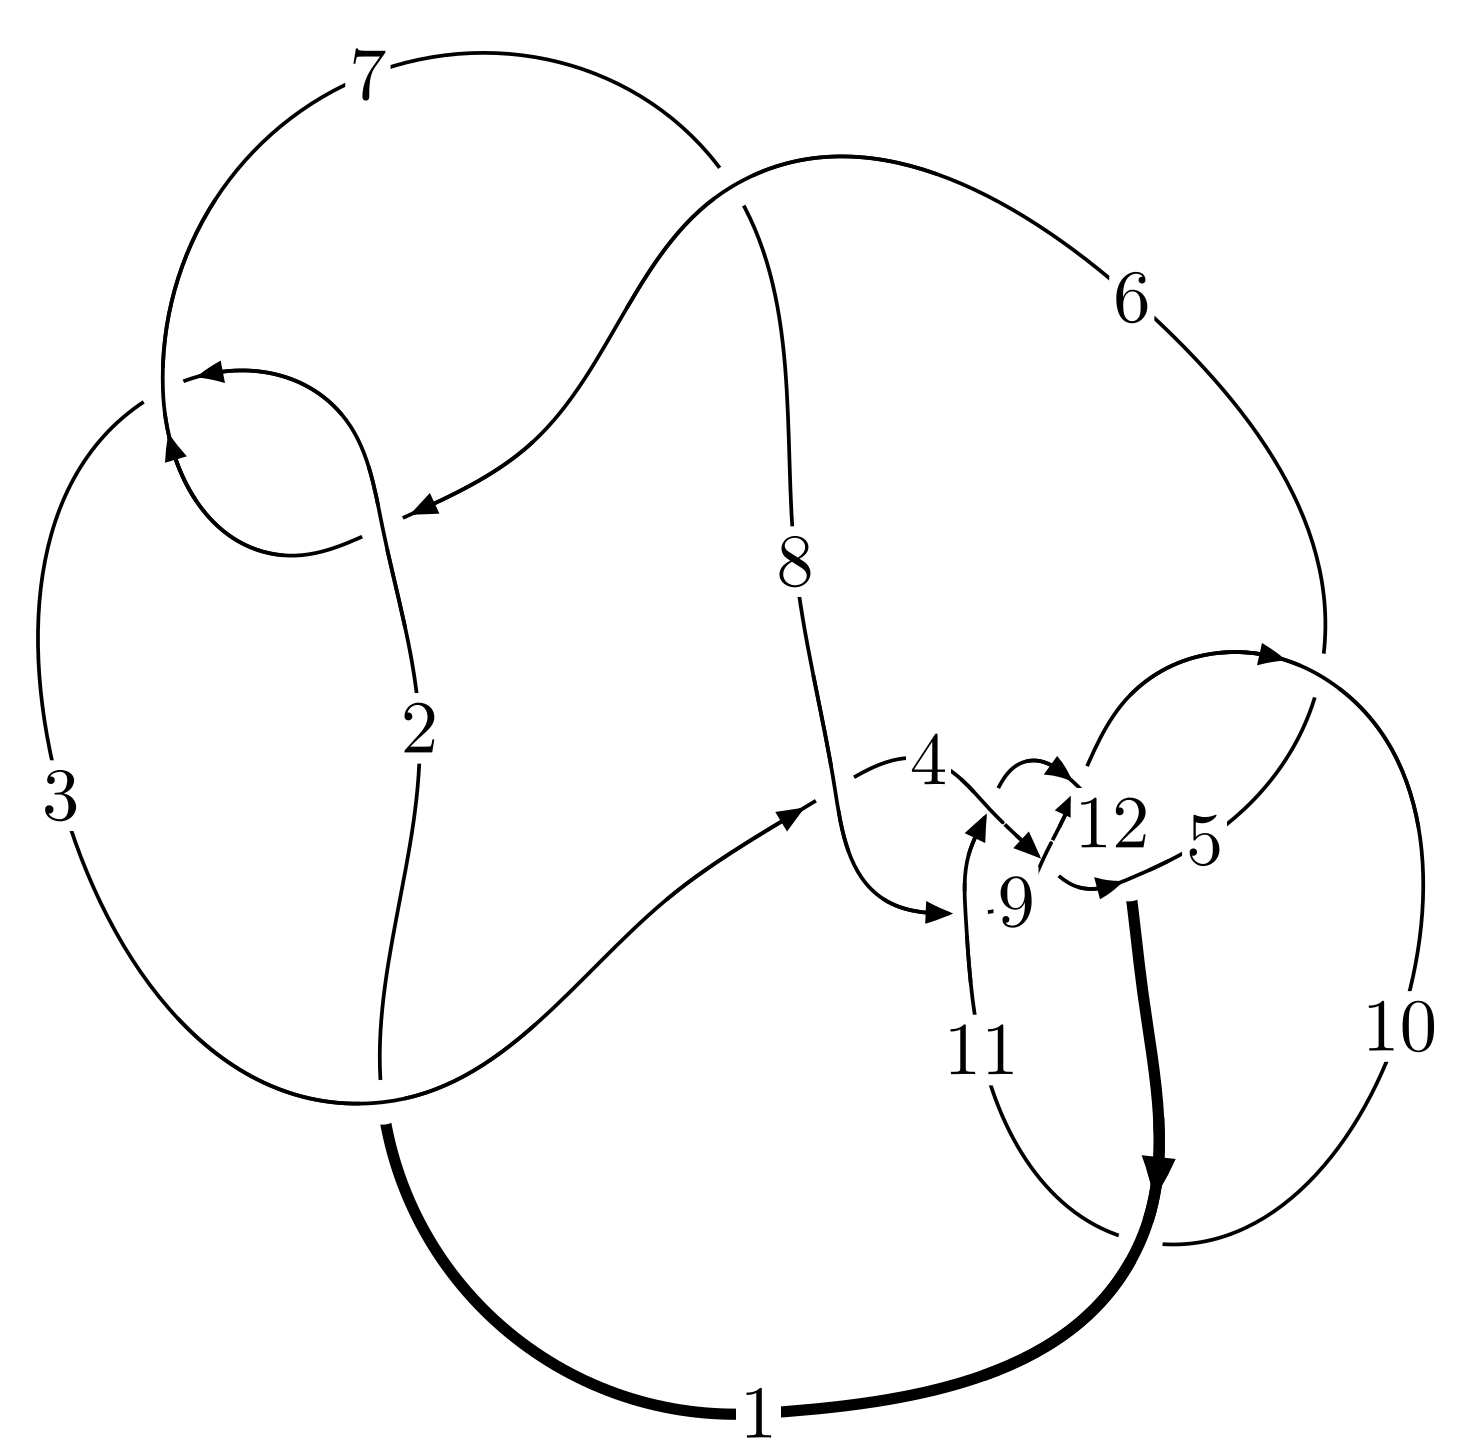
\includegraphics[width=112pt]{../../../GIT/diagram.site/Diagrams/png/1297_12a_0496.png}\\
\ \ \ A knot diagram\footnotemark}&
\allowdisplaybreaks
\textbf{Linearized knot diagam} \\
\cline{2-2}
 &
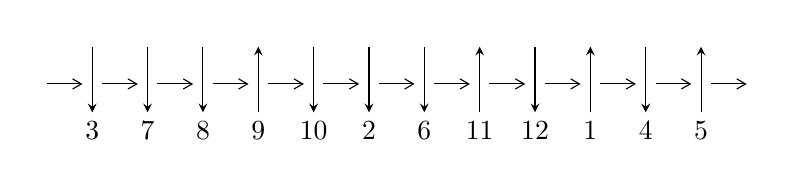
\begin{tikzpicture}[x=20pt, y=17pt]
	% nodes
	\node (C0) at (0, 0) {};
	\node (C1) at (1, 0) {};
	\node (C1U) at (1, +1) {};
	\node (C1D) at (1, -1) {3};

	\node (C2) at (2, 0) {};
	\node (C2U) at (2, +1) {};
	\node (C2D) at (2, -1) {7};

	\node (C3) at (3, 0) {};
	\node (C3U) at (3, +1) {};
	\node (C3D) at (3, -1) {8};

	\node (C4) at (4, 0) {};
	\node (C4U) at (4, +1) {};
	\node (C4D) at (4, -1) {9};

	\node (C5) at (5, 0) {};
	\node (C5U) at (5, +1) {};
	\node (C5D) at (5, -1) {10};

	\node (C6) at (6, 0) {};
	\node (C6U) at (6, +1) {};
	\node (C6D) at (6, -1) {2};

	\node (C7) at (7, 0) {};
	\node (C7U) at (7, +1) {};
	\node (C7D) at (7, -1) {6};

	\node (C8) at (8, 0) {};
	\node (C8U) at (8, +1) {};
	\node (C8D) at (8, -1) {11};

	\node (C9) at (9, 0) {};
	\node (C9U) at (9, +1) {};
	\node (C9D) at (9, -1) {12};

	\node (C10) at (10, 0) {};
	\node (C10U) at (10, +1) {};
	\node (C10D) at (10, -1) {1};

	\node (C11) at (11, 0) {};
	\node (C11U) at (11, +1) {};
	\node (C11D) at (11, -1) {4};

	\node (C12) at (12, 0) {};
	\node (C12U) at (12, +1) {};
	\node (C12D) at (12, -1) {5};
	\node (C13) at (13, 0) {};

	% arrows
	\draw[->,>={angle 60}]
	(C0) edge (C1) (C1) edge (C2) (C2) edge (C3) (C3) edge (C4) (C4) edge (C5) (C5) edge (C6) (C6) edge (C7) (C7) edge (C8) (C8) edge (C9) (C9) edge (C10) (C10) edge (C11) (C11) edge (C12) (C12) edge (C13) ;	\draw[->,>=stealth]
	(C1U) edge (C1D) (C2U) edge (C2D) (C3U) edge (C3D) (C4D) edge (C4U) (C5U) edge (C5D) (C6U) edge (C6D) (C7U) edge (C7D) (C8D) edge (C8U) (C9U) edge (C9D) (C10D) edge (C10U) (C11U) edge (C11D) (C12D) edge (C12U) ;
	\end{tikzpicture} \\
\hhline{~~} \\& 
\textbf{Solving Sequence} \\ \cline{2-2} 
 &
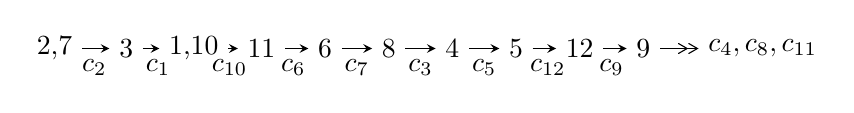
\begin{tikzpicture}[x=23pt, y=7pt]
	% node
	\node (A0) at (-1/8, 0) {2,7};
	\node (A1) at (1, 0) {3};
	\node (A2) at (33/16, 0) {1,10};
	\node (A3) at (25/8, 0) {11};
	\node (A4) at (33/8, 0) {6};
	\node (A5) at (41/8, 0) {8};
	\node (A6) at (49/8, 0) {4};
	\node (A7) at (57/8, 0) {5};
	\node (A8) at (65/8, 0) {12};
	\node (A9) at (73/8, 0) {9};
	\node (C1) at (1/2, -1) {$c_{2}$};
	\node (C2) at (3/2, -1) {$c_{1}$};
	\node (C3) at (21/8, -1) {$c_{10}$};
	\node (C4) at (29/8, -1) {$c_{6}$};
	\node (C5) at (37/8, -1) {$c_{7}$};
	\node (C6) at (45/8, -1) {$c_{3}$};
	\node (C7) at (53/8, -1) {$c_{5}$};
	\node (C8) at (61/8, -1) {$c_{12}$};
	\node (C9) at (69/8, -1) {$c_{9}$};
	\node (A10) at (11, 0) {$c_{4},c_{8},c_{11}$};

	% edge
	\draw[->,>=stealth]	
	(A0) edge (A1) (A1) edge (A2) (A2) edge (A3) (A3) edge (A4) (A4) edge (A5) (A5) edge (A6) (A6) edge (A7) (A7) edge (A8) (A8) edge (A9) ;
	\draw[->>,>={angle 60}]	
	(A9) edge (A10);
\end{tikzpicture} \\ 

\end{tabular} \\

\footnotetext{
The image of knot diagram is generated by the software ``\textbf{Draw programme}" developed by Andrew Bartholomew(\url{http://www.layer8.co.uk/maths/draw/index.htm\#Running-draw}), where we modified some parts for our purpose(\url{https://github.com/CATsTAILs/LinksPainter}).
}\phantom \\ \newline 
\centering \textbf{Ideals for irreducible components\footnotemark of $X_{\text{par}}$} 
 
\begin{align*}
I^u_{1}&=\langle 
-1734730 u^{63}+7359550 u^{62}+\cdots+238897 b+11914608,\\
\phantom{I^u_{1}}&\phantom{= \langle  }-8636494 u^{63}+40140921 u^{62}+\cdots+1672279 a+84242322,\;u^{64}-5 u^{63}+\cdots-46 u+7\rangle \\
I^u_{2}&=\langle 
150 u^{46} a-680138 u^{46}+\cdots-95994 a-523234,\;-6 u^{46} a+4 u^{46}+\cdots+2 a-4,\\
\phantom{I^u_{2}}&\phantom{= \langle  }u^{47}+2 u^{46}+\cdots+6 u^2-1\rangle \\
I^u_{3}&=\langle 
2 u^{19}-3 u^{18}+\cdots+b-3,\;2 u^{19}-2 u^{18}+\cdots+a-1,\;u^{20}-2 u^{19}+\cdots-2 u+1\rangle \\
I^u_{4}&=\langle 
-2 u^2+b- u+1,\;-2 u^2+a- u,\;u^3+u^2-1\rangle \\
I^u_{5}&=\langle 
- u^2+b-2 u,\;- u^2+a- u+1,\;u^3+u^2-1\rangle \\
\\
I^v_{1}&=\langle 
a,\;b-1,\;v+1\rangle \\
\end{align*}
\raggedright * 6 irreducible components of $\dim_{\mathbb{C}}=0$, with total 185 representations.\\
\footnotetext{All coefficients of polynomials are rational numbers. But the coefficients are sometimes approximated in decimal forms when there is not enough margin.}
\newpage
\renewcommand{\arraystretch}{1}
\centering \section*{I. $I^u_{1}= \langle -1.73\times10^{6} u^{63}+7.36\times10^{6} u^{62}+\cdots+2.39\times10^{5} b+1.19\times10^{7},\;-8.64\times10^{6} u^{63}+4.01\times10^{7} u^{62}+\cdots+1.67\times10^{6} a+8.42\times10^{7},\;u^{64}-5 u^{63}+\cdots-46 u+7 \rangle$}
\flushleft \textbf{(i) Arc colorings}\\
\begin{tabular}{m{7pt} m{180pt} m{7pt} m{180pt} }
\flushright $a_{2}=$&$\begin{pmatrix}1\\0\end{pmatrix}$ \\
\flushright $a_{7}=$&$\begin{pmatrix}0\\u\end{pmatrix}$ \\
\flushright $a_{3}=$&$\begin{pmatrix}1\\u^2\end{pmatrix}$ \\
\flushright $a_{1}=$&$\begin{pmatrix}- u^2+1\\- u^4\end{pmatrix}$ \\
\flushright $a_{10}=$&$\begin{pmatrix}5.16451 u^{63}-24.0037 u^{62}+\cdots+303.319 u-50.3758\\7.26141 u^{63}-30.8064 u^{62}+\cdots+292.630 u-49.8734\end{pmatrix}$ \\
\flushright $a_{11}=$&$\begin{pmatrix}2.48151 u^{63}-20.2200 u^{62}+\cdots+322.081 u-53.6177\\-7.81243 u^{63}+18.6263 u^{62}+\cdots+60.5318 u-17.3706\end{pmatrix}$ \\
\flushright $a_{6}=$&$\begin{pmatrix}u\\u\end{pmatrix}$ \\
\flushright $a_{8}=$&$\begin{pmatrix}- u^3\\- u^3+u\end{pmatrix}$ \\
\flushright $a_{4}=$&$\begin{pmatrix}- u^8+u^6- u^4+1\\- u^8+2 u^6-2 u^4+2 u^2\end{pmatrix}$ \\
\flushright $a_{5}=$&$\begin{pmatrix}16.0754 u^{63}-59.9879 u^{62}+\cdots+275.423 u-35.9390\\18.6758 u^{63}-76.4973 u^{62}+\cdots+561.005 u-87.3529\end{pmatrix}$ \\
\flushright $a_{12}=$&$\begin{pmatrix}3.22947 u^{63}-27.3703 u^{62}+\cdots+454.241 u-78.3087\\-10.5895 u^{63}+24.5239 u^{62}+\cdots+149.285 u-35.7643\end{pmatrix}$ \\
\flushright $a_{9}=$&$\begin{pmatrix}2.61568 u^{63}-11.2817 u^{62}+\cdots+143.423 u-21.8542\\1.79666 u^{63}-8.38758 u^{62}+\cdots+99.4670 u-18.3098\end{pmatrix}$\\&\end{tabular}
\flushleft \textbf{(ii) Obstruction class $= -1$}\\~\\
\flushleft \textbf{(iii) Cusp Shapes $= \frac{185551}{238897} u^{63}+\frac{3341470}{238897} u^{62}+\cdots-\frac{143830148}{238897} u+\frac{29363823}{238897}$}\\~\\
\newpage\renewcommand{\arraystretch}{1}
\flushleft \textbf{(iv) u-Polynomials at the component}\newline \\
\begin{tabular}{m{50pt}|m{274pt}}
Crossings & \hspace{64pt}u-Polynomials at each crossing \\
\hline $$\begin{aligned}c_{1},c_{7}\end{aligned}$$&$\begin{aligned}
&u^{64}+23 u^{63}+\cdots+464 u+49
\end{aligned}$\\
\hline $$\begin{aligned}c_{2},c_{6}\end{aligned}$$&$\begin{aligned}
&u^{64}-5 u^{63}+\cdots-46 u+7
\end{aligned}$\\
\hline $$\begin{aligned}c_{3}\end{aligned}$$&$\begin{aligned}
&u^{64}+7 u^{63}+\cdots-34358 u+14287
\end{aligned}$\\
\hline $$\begin{aligned}c_{4},c_{12}\end{aligned}$$&$\begin{aligned}
&u^{64}+3 u^{63}+\cdots- u-1
\end{aligned}$\\
\hline $$\begin{aligned}c_{5},c_{11}\end{aligned}$$&$\begin{aligned}
&u^{64}+2 u^{63}+\cdots-2 u+1
\end{aligned}$\\
\hline $$\begin{aligned}c_{8},c_{10}\end{aligned}$$&$\begin{aligned}
&u^{64}-10 u^{63}+\cdots+14 u+1
\end{aligned}$\\
\hline $$\begin{aligned}c_{9}\end{aligned}$$&$\begin{aligned}
&u^{64}-34 u^{63}+\cdots+22 u-7
\end{aligned}$\\
\hline
\end{tabular}\\~\\
\newpage\renewcommand{\arraystretch}{1}
\flushleft \textbf{(v) Riley Polynomials at the component}\newline \\
\begin{tabular}{m{50pt}|m{274pt}}
Crossings & \hspace{64pt}Riley Polynomials at each crossing \\
\hline $$\begin{aligned}c_{1},c_{7}\end{aligned}$$&$\begin{aligned}
&y^{64}+41 y^{63}+\cdots+127704 y+2401
\end{aligned}$\\
\hline $$\begin{aligned}c_{2},c_{6}\end{aligned}$$&$\begin{aligned}
&y^{64}-23 y^{63}+\cdots-464 y+49
\end{aligned}$\\
\hline $$\begin{aligned}c_{3}\end{aligned}$$&$\begin{aligned}
&y^{64}-21 y^{63}+\cdots-4975613696 y+204118369
\end{aligned}$\\
\hline $$\begin{aligned}c_{4},c_{12}\end{aligned}$$&$\begin{aligned}
&y^{64}-35 y^{63}+\cdots-77 y+1
\end{aligned}$\\
\hline $$\begin{aligned}c_{5},c_{11}\end{aligned}$$&$\begin{aligned}
&y^{64}-14 y^{63}+\cdots-14 y+1
\end{aligned}$\\
\hline $$\begin{aligned}c_{8},c_{10}\end{aligned}$$&$\begin{aligned}
&y^{64}-26 y^{63}+\cdots-118 y+1
\end{aligned}$\\
\hline $$\begin{aligned}c_{9}\end{aligned}$$&$\begin{aligned}
&y^{64}+22 y^{62}+\cdots-946 y+49
\end{aligned}$\\
\hline
\end{tabular}\\~\\
\newpage\flushleft \textbf{(vi) Complex Volumes and Cusp Shapes}
$$\begin{array}{c|c|c}  
\text{Solutions to }I^u_{1}& \I (\text{vol} + \sqrt{-1}CS) & \text{Cusp shape}\\
 \hline 
\begin{aligned}
u &= -0.697962 + 0.708130 I \\
a &= -1.67956 - 1.76520 I \\
b &= -0.852517 - 0.546831 I\end{aligned}
 & \phantom{-}3.23555 - 0.09263 I & \phantom{-0.000000 } 0 \\ \hline\begin{aligned}
u &= -0.697962 - 0.708130 I \\
a &= -1.67956 + 1.76520 I \\
b &= -0.852517 + 0.546831 I\end{aligned}
 & \phantom{-}3.23555 + 0.09263 I & \phantom{-0.000000 } 0 \\ \hline\begin{aligned}
u &= \phantom{-}1.00820\phantom{ +0.000000I} \\
a &= \phantom{-}1.45537\phantom{ +0.000000I} \\
b &= \phantom{-}2.94663\phantom{ +0.000000I}\end{aligned}
 & -1.74441\phantom{ +0.000000I} & -5.99190\phantom{ +0.000000I} \\ \hline\begin{aligned}
u &= \phantom{-}0.639156 + 0.782956 I \\
a &= -1.10014 + 2.11562 I \\
b &= -1.50171 + 1.10683 I\end{aligned}
 & \phantom{-}2.98257 + 5.54336 I & \phantom{-0.000000 } 0. - 6.27222 I \\ \hline\begin{aligned}
u &= \phantom{-}0.639156 - 0.782956 I \\
a &= -1.10014 - 2.11562 I \\
b &= -1.50171 - 1.10683 I\end{aligned}
 & \phantom{-}2.98257 - 5.54336 I & \phantom{-0.000000 -}0. + 6.27222 I \\ \hline\begin{aligned}
u &= \phantom{-}0.728093 + 0.711367 I \\
a &= \phantom{-}0.68572 + 1.76281 I \\
b &= -0.46330 + 1.96744 I\end{aligned}
 & \phantom{-}3.52720 - 0.00884 I & \phantom{-0.000000 } 0 \\ \hline\begin{aligned}
u &= \phantom{-}0.728093 - 0.711367 I \\
a &= \phantom{-}0.68572 - 1.76281 I \\
b &= -0.46330 - 1.96744 I\end{aligned}
 & \phantom{-}3.52720 + 0.00884 I & \phantom{-0.000000 } 0 \\ \hline\begin{aligned}
u &= \phantom{-}0.572354 + 0.786065 I \\
a &= -0.051150 + 0.959296 I \\
b &= -0.059433 + 0.598116 I\end{aligned}
 & \phantom{-}2.29221 + 1.37861 I & \phantom{-}3.68261 - 1.26528 I \\ \hline\begin{aligned}
u &= \phantom{-}0.572354 - 0.786065 I \\
a &= -0.051150 - 0.959296 I \\
b &= -0.059433 - 0.598116 I\end{aligned}
 & \phantom{-}2.29221 - 1.37861 I & \phantom{-}3.68261 + 1.26528 I \\ \hline\begin{aligned}
u &= \phantom{-}0.804285 + 0.524113 I \\
a &= \phantom{-}0.190288 - 1.042600 I \\
b &= \phantom{-}1.091820 - 0.891582 I\end{aligned}
 & \phantom{-}1.03742 - 3.37211 I & -1.80469 + 6.78145 I\\
 \hline 
 \end{array}$$\newpage$$\begin{array}{c|c|c}  
\text{Solutions to }I^u_{1}& \I (\text{vol} + \sqrt{-1}CS) & \text{Cusp shape}\\
 \hline 
\begin{aligned}
u &= \phantom{-}0.804285 - 0.524113 I \\
a &= \phantom{-}0.190288 + 1.042600 I \\
b &= \phantom{-}1.091820 + 0.891582 I\end{aligned}
 & \phantom{-}1.03742 + 3.37211 I & -1.80469 - 6.78145 I \\ \hline\begin{aligned}
u &= \phantom{-}0.634325 + 0.833636 I \\
a &= \phantom{-}1.54312 - 2.00028 I \\
b &= \phantom{-}1.54828 - 0.43921 I\end{aligned}
 & \phantom{-}1.2900 + 14.4309 I & \phantom{-0.000000 } 0 \\ \hline\begin{aligned}
u &= \phantom{-}0.634325 - 0.833636 I \\
a &= \phantom{-}1.54312 + 2.00028 I \\
b &= \phantom{-}1.54828 + 0.43921 I\end{aligned}
 & \phantom{-}1.2900 - 14.4309 I & \phantom{-0.000000 } 0 \\ \hline\begin{aligned}
u &= -0.932588 + 0.007398 I \\
a &= \phantom{-}0.415698 + 0.467945 I \\
b &= -0.186759 - 0.248263 I\end{aligned}
 & -1.339460 + 0.449150 I & -6.56145 - 1.67611 I \\ \hline\begin{aligned}
u &= -0.932588 - 0.007398 I \\
a &= \phantom{-}0.415698 - 0.467945 I \\
b &= -0.186759 + 0.248263 I\end{aligned}
 & -1.339460 - 0.449150 I & -6.56145 + 1.67611 I \\ \hline\begin{aligned}
u &= -1.071850 + 0.068659 I \\
a &= \phantom{-}0.669015 + 1.069670 I \\
b &= \phantom{-}1.293700 + 0.264092 I\end{aligned}
 & -2.98372 + 5.03113 I & \phantom{-0.000000 } 0 \\ \hline\begin{aligned}
u &= -1.071850 - 0.068659 I \\
a &= \phantom{-}0.669015 - 1.069670 I \\
b &= \phantom{-}1.293700 - 0.264092 I\end{aligned}
 & -2.98372 - 5.03113 I & \phantom{-0.000000 } 0 \\ \hline\begin{aligned}
u &= \phantom{-}1.07680\phantom{ +0.000000I} \\
a &= -0.786660\phantom{ +0.000000I} \\
b &= -1.75843\phantom{ +0.000000I}\end{aligned}
 & -6.33617\phantom{ +0.000000I} & -14.1800\phantom{ +0.000000I} \\ \hline\begin{aligned}
u &= -0.592507 + 0.702795 I \\
a &= \phantom{-}0.752269 + 0.978771 I \\
b &= \phantom{-}0.174748 + 0.081898 I\end{aligned}
 & -1.043970 - 0.946914 I & -6.98595 + 0. I\phantom{ +0.000000I} \\ \hline\begin{aligned}
u &= -0.592507 - 0.702795 I \\
a &= \phantom{-}0.752269 - 0.978771 I \\
b &= \phantom{-}0.174748 - 0.081898 I\end{aligned}
 & -1.043970 + 0.946914 I & -6.98595 + 0. I\phantom{ +0.000000I}\\
 \hline 
 \end{array}$$\newpage$$\begin{array}{c|c|c}  
\text{Solutions to }I^u_{1}& \I (\text{vol} + \sqrt{-1}CS) & \text{Cusp shape}\\
 \hline 
\begin{aligned}
u &= \phantom{-}0.736786 + 0.817581 I \\
a &= \phantom{-}0.149009 - 1.133040 I \\
b &= \phantom{-}0.832202 - 0.663254 I\end{aligned}
 & \phantom{-}4.13608 - 1.87912 I & \phantom{-0.000000 } 0 \\ \hline\begin{aligned}
u &= \phantom{-}0.736786 - 0.817581 I \\
a &= \phantom{-}0.149009 + 1.133040 I \\
b &= \phantom{-}0.832202 + 0.663254 I\end{aligned}
 & \phantom{-}4.13608 + 1.87912 I & \phantom{-0.000000 } 0 \\ \hline\begin{aligned}
u &= -1.117060 + 0.109814 I \\
a &= -0.807439 - 0.795984 I \\
b &= -2.03240 - 0.10781 I\end{aligned}
 & -5.2527 + 13.7489 I & \phantom{-0.000000 } 0 \\ \hline\begin{aligned}
u &= -1.117060 - 0.109814 I \\
a &= -0.807439 + 0.795984 I \\
b &= -2.03240 + 0.10781 I\end{aligned}
 & -5.2527 - 13.7489 I & \phantom{-0.000000 } 0 \\ \hline\begin{aligned}
u &= -0.856164 + 0.736535 I \\
a &= -0.84854 - 2.26839 I \\
b &= -1.46492 - 1.86228 I\end{aligned}
 & \phantom{-}6.33526 + 4.44087 I & \phantom{-0.000000 } 0 \\ \hline\begin{aligned}
u &= -0.856164 - 0.736535 I \\
a &= -0.84854 + 2.26839 I \\
b &= -1.46492 + 1.86228 I\end{aligned}
 & \phantom{-}6.33526 - 4.44087 I & \phantom{-0.000000 } 0 \\ \hline\begin{aligned}
u &= -0.868762 + 0.731876 I \\
a &= -2.00888 - 1.13797 I \\
b &= -2.31883 - 0.53167 I\end{aligned}
 & \phantom{-}6.29588 + 1.13543 I & \phantom{-0.000000 } 0 \\ \hline\begin{aligned}
u &= -0.868762 - 0.731876 I \\
a &= -2.00888 + 1.13797 I \\
b &= -2.31883 + 0.53167 I\end{aligned}
 & \phantom{-}6.29588 - 1.13543 I & \phantom{-0.000000 } 0 \\ \hline\begin{aligned}
u &= -1.15307\phantom{ +0.000000I} \\
a &= \phantom{-}0.601343\phantom{ +0.000000I} \\
b &= \phantom{-}0.930830\phantom{ +0.000000I}\end{aligned}
 & -3.58190\phantom{ +0.000000I} & \phantom{-0.000000 } 0 \\ \hline\begin{aligned}
u &= \phantom{-}0.986087 + 0.603160 I \\
a &= \phantom{-}0.759306 - 0.700975 I \\
b &= \phantom{-}0.609793 + 0.181630 I\end{aligned}
 & \phantom{-}0.175719 - 1.083750 I & \phantom{-0.000000 } 0\\
 \hline 
 \end{array}$$\newpage$$\begin{array}{c|c|c}  
\text{Solutions to }I^u_{1}& \I (\text{vol} + \sqrt{-1}CS) & \text{Cusp shape}\\
 \hline 
\begin{aligned}
u &= \phantom{-}0.986087 - 0.603160 I \\
a &= \phantom{-}0.759306 + 0.700975 I \\
b &= \phantom{-}0.609793 - 0.181630 I\end{aligned}
 & \phantom{-}0.175719 + 1.083750 I & \phantom{-0.000000 } 0 \\ \hline\begin{aligned}
u &= \phantom{-}1.062550 + 0.468285 I \\
a &= -0.200162 + 0.267131 I \\
b &= -1.041540 + 0.047587 I\end{aligned}
 & -1.95009 - 8.80692 I & \phantom{-0.000000 } 0 \\ \hline\begin{aligned}
u &= \phantom{-}1.062550 - 0.468285 I \\
a &= -0.200162 - 0.267131 I \\
b &= -1.041540 - 0.047587 I\end{aligned}
 & -1.95009 + 8.80692 I & \phantom{-0.000000 } 0 \\ \hline\begin{aligned}
u &= -0.846265 + 0.805401 I \\
a &= \phantom{-}1.84643 + 0.87650 I \\
b &= \phantom{-}1.95412 - 0.27824 I\end{aligned}
 & \phantom{-}6.28695 - 5.68542 I & \phantom{-0.000000 } 0 \\ \hline\begin{aligned}
u &= -0.846265 - 0.805401 I \\
a &= \phantom{-}1.84643 - 0.87650 I \\
b &= \phantom{-}1.95412 + 0.27824 I\end{aligned}
 & \phantom{-}6.28695 + 5.68542 I & \phantom{-0.000000 } 0 \\ \hline\begin{aligned}
u &= \phantom{-}1.044360 + 0.535925 I \\
a &= -0.297767 - 0.010643 I \\
b &= \phantom{-}0.287388 - 1.086830 I\end{aligned}
 & -2.64693 + 6.82839 I & \phantom{-0.000000 } 0 \\ \hline\begin{aligned}
u &= \phantom{-}1.044360 - 0.535925 I \\
a &= -0.297767 + 0.010643 I \\
b &= \phantom{-}0.287388 + 1.086830 I\end{aligned}
 & -2.64693 - 6.82839 I & \phantom{-0.000000 } 0 \\ \hline\begin{aligned}
u &= \phantom{-}0.965327 + 0.681396 I \\
a &= -1.83686 - 0.09440 I \\
b &= -1.57566 - 1.07217 I\end{aligned}
 & \phantom{-}2.80623 - 5.34875 I & \phantom{-0.000000 } 0 \\ \hline\begin{aligned}
u &= \phantom{-}0.965327 - 0.681396 I \\
a &= -1.83686 + 0.09440 I \\
b &= -1.57566 + 1.07217 I\end{aligned}
 & \phantom{-}2.80623 + 5.34875 I & \phantom{-0.000000 } 0 \\ \hline\begin{aligned}
u &= -0.982823 + 0.674637 I \\
a &= -1.31717 - 1.51958 I \\
b &= -2.48194 - 2.08681 I\end{aligned}
 & \phantom{-}2.37380 + 5.42471 I & \phantom{-0.000000 } 0\\
 \hline 
 \end{array}$$\newpage$$\begin{array}{c|c|c}  
\text{Solutions to }I^u_{1}& \I (\text{vol} + \sqrt{-1}CS) & \text{Cusp shape}\\
 \hline 
\begin{aligned}
u &= -0.982823 - 0.674637 I \\
a &= -1.31717 + 1.51958 I \\
b &= -2.48194 + 2.08681 I\end{aligned}
 & \phantom{-}2.37380 - 5.42471 I & \phantom{-0.000000 } 0 \\ \hline\begin{aligned}
u &= -1.172950 + 0.233278 I \\
a &= -0.046370 + 0.198660 I \\
b &= \phantom{-}0.219915 + 0.658412 I\end{aligned}
 & -3.53632 - 1.31927 I & \phantom{-0.000000 } 0 \\ \hline\begin{aligned}
u &= -1.172950 - 0.233278 I \\
a &= -0.046370 - 0.198660 I \\
b &= \phantom{-}0.219915 - 0.658412 I\end{aligned}
 & -3.53632 + 1.31927 I & \phantom{-0.000000 } 0 \\ \hline\begin{aligned}
u &= -0.904136 + 0.786401 I \\
a &= \phantom{-}0.45867 + 2.05749 I \\
b &= \phantom{-}1.62123 + 1.88253 I\end{aligned}
 & \phantom{-}6.10887 + 11.63470 I & \phantom{-0.000000 } 0 \\ \hline\begin{aligned}
u &= -0.904136 - 0.786401 I \\
a &= \phantom{-}0.45867 - 2.05749 I \\
b &= \phantom{-}1.62123 - 1.88253 I\end{aligned}
 & \phantom{-}6.10887 - 11.63470 I & \phantom{-0.000000 } 0 \\ \hline\begin{aligned}
u &= -1.016970 + 0.654432 I \\
a &= \phantom{-}0.747567 + 0.699678 I \\
b &= \phantom{-}1.53161 + 1.07598 I\end{aligned}
 & -2.27025 + 6.19345 I & \phantom{-0.000000 } 0 \\ \hline\begin{aligned}
u &= -1.016970 - 0.654432 I \\
a &= \phantom{-}0.747567 - 0.699678 I \\
b &= \phantom{-}1.53161 - 1.07598 I\end{aligned}
 & -2.27025 - 6.19345 I & \phantom{-0.000000 } 0 \\ \hline\begin{aligned}
u &= \phantom{-}0.303108 + 0.722084 I \\
a &= \phantom{-}0.781154 - 0.316034 I \\
b &= -0.878500 + 0.638191 I\end{aligned}
 & -0.52027 - 11.41630 I & -2.49256 + 8.08162 I \\ \hline\begin{aligned}
u &= \phantom{-}0.303108 - 0.722084 I \\
a &= \phantom{-}0.781154 + 0.316034 I \\
b &= -0.878500 - 0.638191 I\end{aligned}
 & -0.52027 + 11.41630 I & -2.49256 - 8.08162 I \\ \hline\begin{aligned}
u &= \phantom{-}0.981513 + 0.732663 I \\
a &= \phantom{-}1.019970 - 0.631499 I \\
b &= \phantom{-}1.48785 - 0.02952 I\end{aligned}
 & \phantom{-}3.38294 - 3.93081 I & \phantom{-0.000000 } 0\\
 \hline 
 \end{array}$$\newpage$$\begin{array}{c|c|c}  
\text{Solutions to }I^u_{1}& \I (\text{vol} + \sqrt{-1}CS) & \text{Cusp shape}\\
 \hline 
\begin{aligned}
u &= \phantom{-}0.981513 - 0.732663 I \\
a &= \phantom{-}1.019970 + 0.631499 I \\
b &= \phantom{-}1.48785 + 0.02952 I\end{aligned}
 & \phantom{-}3.38294 + 3.93081 I & \phantom{-0.000000 } 0 \\ \hline\begin{aligned}
u &= \phantom{-}0.154501 + 0.750893 I \\
a &= \phantom{-}0.336028 + 0.604708 I \\
b &= -0.436498 - 0.329752 I\end{aligned}
 & \phantom{-}0.75067 + 4.55551 I & \phantom{-}2.40157 - 10.29146 I \\ \hline\begin{aligned}
u &= \phantom{-}0.154501 - 0.750893 I \\
a &= \phantom{-}0.336028 - 0.604708 I \\
b &= -0.436498 + 0.329752 I\end{aligned}
 & \phantom{-}0.75067 - 4.55551 I & \phantom{-}2.40157 + 10.29146 I \\ \hline\begin{aligned}
u &= \phantom{-}1.023840 + 0.691795 I \\
a &= -1.96311 + 1.54995 I \\
b &= -2.78367 + 1.14339 I\end{aligned}
 & \phantom{-}1.82985 - 11.12330 I & \phantom{-0.000000 } 0 \\ \hline\begin{aligned}
u &= \phantom{-}1.023840 - 0.691795 I \\
a &= -1.96311 - 1.54995 I \\
b &= -2.78367 - 1.14339 I\end{aligned}
 & \phantom{-}1.82985 + 11.12330 I & \phantom{-0.000000 } 0 \\ \hline\begin{aligned}
u &= \phantom{-}1.052550 + 0.676673 I \\
a &= -0.954979 + 0.296922 I \\
b &= -1.312160 + 0.307764 I\end{aligned}
 & \phantom{-}0.87367 - 6.91136 I & \phantom{-0.000000 } 0 \\ \hline\begin{aligned}
u &= \phantom{-}1.052550 - 0.676673 I \\
a &= -0.954979 - 0.296922 I \\
b &= -1.312160 - 0.307764 I\end{aligned}
 & \phantom{-}0.87367 + 6.91136 I & \phantom{-0.000000 } 0 \\ \hline\begin{aligned}
u &= \phantom{-}1.043210 + 0.709927 I \\
a &= \phantom{-}1.67256 - 1.84369 I \\
b &= \phantom{-}2.98654 - 1.78795 I\end{aligned}
 & \phantom{-}0.0504 - 20.2068 I & \phantom{-0.000000 } 0 \\ \hline\begin{aligned}
u &= \phantom{-}1.043210 - 0.709927 I \\
a &= \phantom{-}1.67256 + 1.84369 I \\
b &= \phantom{-}2.98654 + 1.78795 I\end{aligned}
 & \phantom{-}0.0504 + 20.2068 I & \phantom{-0.000000 } 0 \\ \hline\begin{aligned}
u &= \phantom{-}0.361556 + 0.559052 I \\
a &= -0.400060 - 0.573207 I \\
b &= \phantom{-}1.044170 - 0.600052 I\end{aligned}
 & \phantom{-}1.50411 - 3.41073 I & \phantom{-}3.06252 + 7.09437 I\\
 \hline 
 \end{array}$$\newpage$$\begin{array}{c|c|c}  
\text{Solutions to }I^u_{1}& \I (\text{vol} + \sqrt{-1}CS) & \text{Cusp shape}\\
 \hline 
\begin{aligned}
u &= \phantom{-}0.361556 - 0.559052 I \\
a &= -0.400060 + 0.573207 I \\
b &= \phantom{-}1.044170 + 0.600052 I\end{aligned}
 & \phantom{-}1.50411 + 3.41073 I & \phantom{-}3.06252 - 7.09437 I \\ \hline\begin{aligned}
u &= -0.640733\phantom{ +0.000000I} \\
a &= \phantom{-}0.559622\phantom{ +0.000000I} \\
b &= -0.336776\phantom{ +0.000000I}\end{aligned}
 & -0.999154\phantom{ +0.000000I} & -9.88350\phantom{ +0.000000I} \\ \hline\begin{aligned}
u &= \phantom{-}0.320846 + 0.345616 I \\
a &= \phantom{-}0.856259 - 0.836701 I \\
b &= \phantom{-}0.815333 + 0.325629 I\end{aligned}
 & \phantom{-}1.85294 + 0.24098 I & \phantom{-}3.67461 + 0.64977 I \\ \hline\begin{aligned}
u &= \phantom{-}0.320846 - 0.345616 I \\
a &= \phantom{-}0.856259 + 0.836701 I \\
b &= \phantom{-}0.815333 - 0.325629 I\end{aligned}
 & \phantom{-}1.85294 - 0.24098 I & \phantom{-}3.67461 - 0.64977 I\\
 \hline 
 \end{array}$$\newpage\newpage\renewcommand{\arraystretch}{1}
\centering \section*{II. $I^u_{2}= \langle 150 u^{46} a-680138 u^{46}+\cdots-95994 a-523234,\;-6 u^{46} a+4 u^{46}+\cdots+2 a-4,\;u^{47}+2 u^{46}+\cdots+6 u^2-1 \rangle$}
\flushleft \textbf{(i) Arc colorings}\\
\begin{tabular}{m{7pt} m{180pt} m{7pt} m{180pt} }
\flushright $a_{2}=$&$\begin{pmatrix}1\\0\end{pmatrix}$ \\
\flushright $a_{7}=$&$\begin{pmatrix}0\\u\end{pmatrix}$ \\
\flushright $a_{3}=$&$\begin{pmatrix}1\\u^2\end{pmatrix}$ \\
\flushright $a_{1}=$&$\begin{pmatrix}- u^2+1\\- u^4\end{pmatrix}$ \\
\flushright $a_{10}=$&$\begin{pmatrix}a\\-0.000413819 a u^{46}+1.87636 u^{46}+\cdots+0.264828 a+1.44350\end{pmatrix}$ \\
\flushright $a_{11}=$&$\begin{pmatrix}-0.312516 a u^{46}-2.77156 u^{46}+\cdots+1.59798 a+2.72797\\0.149146 a u^{46}-1.41248 u^{46}+\cdots+0.312516 a+4.77156\end{pmatrix}$ \\
\flushright $a_{6}=$&$\begin{pmatrix}u\\u\end{pmatrix}$ \\
\flushright $a_{8}=$&$\begin{pmatrix}- u^3\\- u^3+u\end{pmatrix}$ \\
\flushright $a_{4}=$&$\begin{pmatrix}- u^8+u^6- u^4+1\\- u^8+2 u^6-2 u^4+2 u^2\end{pmatrix}$ \\
\flushright $a_{5}=$&$\begin{pmatrix}-0.368892 a u^{46}+0.918130 u^{46}+\cdots+1.87636 a+1.91354\\-0.640937 a u^{46}+1.83838 u^{46}+\cdots+1.17418 a+1.06763\end{pmatrix}$ \\
\flushright $a_{12}=$&$\begin{pmatrix}-0.205293 a u^{46}-2.92275 u^{46}+\cdots+1.65932 a+1.52194\\0.251020 a u^{46}-1.41523 u^{46}+\cdots+0.0771994 a+3.97178\end{pmatrix}$ \\
\flushright $a_{9}=$&$\begin{pmatrix}-0.503113 a u^{46}+2.92316 u^{46}+\cdots+2.81239 a-1.78677\\-0.111028 a u^{46}+2.22787 u^{46}+\cdots+1.45331 a-3.31010\end{pmatrix}$\\&\end{tabular}
\flushleft \textbf{(ii) Obstruction class $= -1$}\\~\\
\flushleft \textbf{(iii) Cusp Shapes $= - u^{46}-6 u^{45}+\cdots-25 u-17$}\\~\\
\newpage\renewcommand{\arraystretch}{1}
\flushleft \textbf{(iv) u-Polynomials at the component}\newline \\
\begin{tabular}{m{50pt}|m{274pt}}
Crossings & \hspace{64pt}u-Polynomials at each crossing \\
\hline $$\begin{aligned}c_{1},c_{7}\end{aligned}$$&$\begin{aligned}
&(u^{47}+16 u^{46}+\cdots+12 u+1)^{2}
\end{aligned}$\\
\hline $$\begin{aligned}c_{2},c_{6}\end{aligned}$$&$\begin{aligned}
&(u^{47}+2 u^{46}+\cdots+6 u^2-1)^{2}
\end{aligned}$\\
\hline $$\begin{aligned}c_{3}\end{aligned}$$&$\begin{aligned}
&(u^{47}-2 u^{46}+\cdots+122 u-37)^{2}
\end{aligned}$\\
\hline $$\begin{aligned}c_{4},c_{12}\end{aligned}$$&$\begin{aligned}
&u^{94}+10 u^{92}+\cdots-7 u+1
\end{aligned}$\\
\hline $$\begin{aligned}c_{5},c_{11}\end{aligned}$$&$\begin{aligned}
&u^{94}-4 u^{92}+\cdots-18201 u+761
\end{aligned}$\\
\hline $$\begin{aligned}c_{8},c_{10}\end{aligned}$$&$\begin{aligned}
&u^{94}+7 u^{93}+\cdots+74 u+19
\end{aligned}$\\
\hline $$\begin{aligned}c_{9}\end{aligned}$$&$\begin{aligned}
&(u^{47}+23 u^{46}+\cdots+12 u+8)^{2}
\end{aligned}$\\
\hline
\end{tabular}\\~\\
\newpage\renewcommand{\arraystretch}{1}
\flushleft \textbf{(v) Riley Polynomials at the component}\newline \\
\begin{tabular}{m{50pt}|m{274pt}}
Crossings & \hspace{64pt}Riley Polynomials at each crossing \\
\hline $$\begin{aligned}c_{1},c_{7}\end{aligned}$$&$\begin{aligned}
&(y^{47}+32 y^{46}+\cdots+12 y-1)^{2}
\end{aligned}$\\
\hline $$\begin{aligned}c_{2},c_{6}\end{aligned}$$&$\begin{aligned}
&(y^{47}-16 y^{46}+\cdots+12 y-1)^{2}
\end{aligned}$\\
\hline $$\begin{aligned}c_{3}\end{aligned}$$&$\begin{aligned}
&(y^{47}-16 y^{46}+\cdots+37824 y-1369)^{2}
\end{aligned}$\\
\hline $$\begin{aligned}c_{4},c_{12}\end{aligned}$$&$\begin{aligned}
&y^{94}+20 y^{93}+\cdots+9 y+1
\end{aligned}$\\
\hline $$\begin{aligned}c_{5},c_{11}\end{aligned}$$&$\begin{aligned}
&y^{94}-8 y^{93}+\cdots-190343767 y+579121
\end{aligned}$\\
\hline $$\begin{aligned}c_{8},c_{10}\end{aligned}$$&$\begin{aligned}
&y^{94}+33 y^{93}+\cdots-11366 y+361
\end{aligned}$\\
\hline $$\begin{aligned}c_{9}\end{aligned}$$&$\begin{aligned}
&(y^{47}-7 y^{46}+\cdots+1424 y-64)^{2}
\end{aligned}$\\
\hline
\end{tabular}\\~\\
\newpage\flushleft \textbf{(vi) Complex Volumes and Cusp Shapes}
$$\begin{array}{c|c|c}  
\text{Solutions to }I^u_{2}& \I (\text{vol} + \sqrt{-1}CS) & \text{Cusp shape}\\
 \hline 
\begin{aligned}
u &= -0.776349 + 0.661422 I \\
a &= \phantom{-}0.758981 + 0.193716 I \\
b &= \phantom{-}1.77645 + 0.49361 I\end{aligned}
 & \phantom{-}1.10849 + 5.40536 I & -0.41152 - 9.36246 I \\ \hline\begin{aligned}
u &= -0.776349 + 0.661422 I \\
a &= \phantom{-}0.54263 - 3.15148 I \\
b &= -0.76174 - 2.41245 I\end{aligned}
 & \phantom{-}1.10849 + 5.40536 I & -0.41152 - 9.36246 I \\ \hline\begin{aligned}
u &= -0.776349 - 0.661422 I \\
a &= \phantom{-}0.758981 - 0.193716 I \\
b &= \phantom{-}1.77645 - 0.49361 I\end{aligned}
 & \phantom{-}1.10849 - 5.40536 I & -0.41152 + 9.36246 I \\ \hline\begin{aligned}
u &= -0.776349 - 0.661422 I \\
a &= \phantom{-}0.54263 + 3.15148 I \\
b &= -0.76174 + 2.41245 I\end{aligned}
 & \phantom{-}1.10849 - 5.40536 I & -0.41152 + 9.36246 I \\ \hline\begin{aligned}
u &= \phantom{-}1.019790 + 0.092510 I \\
a &= \phantom{-}0.68972 - 1.40592 I \\
b &= \phantom{-}1.70152 - 0.86662 I\end{aligned}
 & -2.43130 - 5.51015 I & -4.82916 + 8.03335 I \\ \hline\begin{aligned}
u &= \phantom{-}1.019790 + 0.092510 I \\
a &= \phantom{-}0.029262 + 0.176413 I \\
b &= \phantom{-}0.12157 - 1.45314 I\end{aligned}
 & -2.43130 - 5.51015 I & -4.82916 + 8.03335 I \\ \hline\begin{aligned}
u &= \phantom{-}1.019790 - 0.092510 I \\
a &= \phantom{-}0.68972 + 1.40592 I \\
b &= \phantom{-}1.70152 + 0.86662 I\end{aligned}
 & -2.43130 + 5.51015 I & -4.82916 - 8.03335 I \\ \hline\begin{aligned}
u &= \phantom{-}1.019790 - 0.092510 I \\
a &= \phantom{-}0.029262 - 0.176413 I \\
b &= \phantom{-}0.12157 + 1.45314 I\end{aligned}
 & -2.43130 + 5.51015 I & -4.82916 - 8.03335 I \\ \hline\begin{aligned}
u &= \phantom{-}0.648071 + 0.723212 I \\
a &= -0.736502 - 0.524748 I \\
b &= -1.243130 + 0.114753 I\end{aligned}
 & -0.49007 + 4.87876 I & -5.65107 - 6.38090 I \\ \hline\begin{aligned}
u &= \phantom{-}0.648071 + 0.723212 I \\
a &= -1.79929 + 2.64042 I \\
b &= -1.93267 + 0.81735 I\end{aligned}
 & -0.49007 + 4.87876 I & -5.65107 - 6.38090 I\\
 \hline 
 \end{array}$$\newpage$$\begin{array}{c|c|c}  
\text{Solutions to }I^u_{2}& \I (\text{vol} + \sqrt{-1}CS) & \text{Cusp shape}\\
 \hline 
\begin{aligned}
u &= \phantom{-}0.648071 - 0.723212 I \\
a &= -0.736502 + 0.524748 I \\
b &= -1.243130 - 0.114753 I\end{aligned}
 & -0.49007 - 4.87876 I & -5.65107 + 6.38090 I \\ \hline\begin{aligned}
u &= \phantom{-}0.648071 - 0.723212 I \\
a &= -1.79929 - 2.64042 I \\
b &= -1.93267 - 0.81735 I\end{aligned}
 & -0.49007 - 4.87876 I & -5.65107 + 6.38090 I \\ \hline\begin{aligned}
u &= -0.681587 + 0.784410 I \\
a &= -0.42546 + 2.27854 I \\
b &= \phantom{-}1.20914 + 1.53709 I\end{aligned}
 & \phantom{-}3.54465 - 5.47609 I & \phantom{-}3.45857 + 5.88892 I \\ \hline\begin{aligned}
u &= -0.681587 + 0.784410 I \\
a &= -1.85767 - 1.81979 I \\
b &= -1.80898 - 0.69665 I\end{aligned}
 & \phantom{-}3.54465 - 5.47609 I & \phantom{-}3.45857 + 5.88892 I \\ \hline\begin{aligned}
u &= -0.681587 - 0.784410 I \\
a &= -0.42546 - 2.27854 I \\
b &= \phantom{-}1.20914 - 1.53709 I\end{aligned}
 & \phantom{-}3.54465 + 5.47609 I & \phantom{-}3.45857 - 5.88892 I \\ \hline\begin{aligned}
u &= -0.681587 - 0.784410 I \\
a &= -1.85767 + 1.81979 I \\
b &= -1.80898 + 0.69665 I\end{aligned}
 & \phantom{-}3.54465 + 5.47609 I & \phantom{-}3.45857 - 5.88892 I \\ \hline\begin{aligned}
u &= -1.048580 + 0.022164 I \\
a &= \phantom{-}0.670100 + 0.764343 I \\
b &= \phantom{-}2.00093 - 0.27133 I\end{aligned}
 & -5.85788 + 4.38390 I & -13.6960 - 5.4679 I \\ \hline\begin{aligned}
u &= -1.048580 + 0.022164 I \\
a &= -1.05745 + 1.50356 I \\
b &= -1.65854 + 1.43422 I\end{aligned}
 & -5.85788 + 4.38390 I & -13.6960 - 5.4679 I \\ \hline\begin{aligned}
u &= -1.048580 - 0.022164 I \\
a &= \phantom{-}0.670100 - 0.764343 I \\
b &= \phantom{-}2.00093 + 0.27133 I\end{aligned}
 & -5.85788 - 4.38390 I & -13.6960 + 5.4679 I \\ \hline\begin{aligned}
u &= -1.048580 - 0.022164 I \\
a &= -1.05745 - 1.50356 I \\
b &= -1.65854 - 1.43422 I\end{aligned}
 & -5.85788 - 4.38390 I & -13.6960 + 5.4679 I\\
 \hline 
 \end{array}$$\newpage$$\begin{array}{c|c|c}  
\text{Solutions to }I^u_{2}& \I (\text{vol} + \sqrt{-1}CS) & \text{Cusp shape}\\
 \hline 
\begin{aligned}
u &= -0.643340 + 0.833331 I \\
a &= -1.20226 - 0.85122 I \\
b &= -1.027200 - 0.118397 I\end{aligned}
 & -0.23631 - 6.14773 I & -6.28409 + 6.42865 I \\ \hline\begin{aligned}
u &= -0.643340 + 0.833331 I \\
a &= \phantom{-}1.43841 + 1.82679 I \\
b &= \phantom{-}1.45781 + 0.21030 I\end{aligned}
 & -0.23631 - 6.14773 I & -6.28409 + 6.42865 I \\ \hline\begin{aligned}
u &= -0.643340 - 0.833331 I \\
a &= -1.20226 + 0.85122 I \\
b &= -1.027200 + 0.118397 I\end{aligned}
 & -0.23631 + 6.14773 I & -6.28409 - 6.42865 I \\ \hline\begin{aligned}
u &= -0.643340 - 0.833331 I \\
a &= \phantom{-}1.43841 - 1.82679 I \\
b &= \phantom{-}1.45781 - 0.21030 I\end{aligned}
 & -0.23631 + 6.14773 I & -6.28409 - 6.42865 I \\ \hline\begin{aligned}
u &= \phantom{-}1.07542\phantom{ +0.000000I} \\
a &= -0.782008 + 0.163949 I \\
b &= -1.74468 + 0.12456 I\end{aligned}
 & -6.33500\phantom{ +0.000000I} & -14.0910\phantom{ +0.000000I} \\ \hline\begin{aligned}
u &= \phantom{-}1.07542\phantom{ +0.000000I} \\
a &= -0.782008 - 0.163949 I \\
b &= -1.74468 - 0.12456 I\end{aligned}
 & -6.33500\phantom{ +0.000000I} & -14.0910\phantom{ +0.000000I} \\ \hline\begin{aligned}
u &= \phantom{-}0.642944 + 0.643850 I \\
a &= -1.078100 - 0.664840 I \\
b &= \phantom{-}0.621290 - 1.023730 I\end{aligned}
 & -1.02865 - 3.62128 I & -7.85432 + 4.03793 I \\ \hline\begin{aligned}
u &= \phantom{-}0.642944 + 0.643850 I \\
a &= \phantom{-}1.48670 - 1.74194 I \\
b &= \phantom{-}1.18147 - 1.47113 I\end{aligned}
 & -1.02865 - 3.62128 I & -7.85432 + 4.03793 I \\ \hline\begin{aligned}
u &= \phantom{-}0.642944 - 0.643850 I \\
a &= -1.078100 + 0.664840 I \\
b &= \phantom{-}0.621290 + 1.023730 I\end{aligned}
 & -1.02865 + 3.62128 I & -7.85432 - 4.03793 I \\ \hline\begin{aligned}
u &= \phantom{-}0.642944 - 0.643850 I \\
a &= \phantom{-}1.48670 + 1.74194 I \\
b &= \phantom{-}1.18147 + 1.47113 I\end{aligned}
 & -1.02865 + 3.62128 I & -7.85432 - 4.03793 I\\
 \hline 
 \end{array}$$\newpage$$\begin{array}{c|c|c}  
\text{Solutions to }I^u_{2}& \I (\text{vol} + \sqrt{-1}CS) & \text{Cusp shape}\\
 \hline 
\begin{aligned}
u &= -0.574541 + 0.684773 I \\
a &= \phantom{-}0.906959 + 0.595184 I \\
b &= \phantom{-}0.189356 - 0.393389 I\end{aligned}
 & -1.09201 - 0.99704 I & -7.43094 + 0.59298 I \\ \hline\begin{aligned}
u &= -0.574541 + 0.684773 I \\
a &= \phantom{-}0.68672 + 1.27674 I \\
b &= \phantom{-}0.036037 + 0.532121 I\end{aligned}
 & -1.09201 - 0.99704 I & -7.43094 + 0.59298 I \\ \hline\begin{aligned}
u &= -0.574541 - 0.684773 I \\
a &= \phantom{-}0.906959 - 0.595184 I \\
b &= \phantom{-}0.189356 + 0.393389 I\end{aligned}
 & -1.09201 + 0.99704 I & -7.43094 - 0.59298 I \\ \hline\begin{aligned}
u &= -0.574541 - 0.684773 I \\
a &= \phantom{-}0.68672 - 1.27674 I \\
b &= \phantom{-}0.036037 - 0.532121 I\end{aligned}
 & -1.09201 + 0.99704 I & -7.43094 - 0.59298 I \\ \hline\begin{aligned}
u &= \phantom{-}1.108130 + 0.117843 I \\
a &= \phantom{-}0.197788 - 0.818395 I \\
b &= \phantom{-}0.958445 - 0.713043 I\end{aligned}
 & -6.80256 - 5.57711 I & -13.3130 + 6.5645 I \\ \hline\begin{aligned}
u &= \phantom{-}1.108130 + 0.117843 I \\
a &= -0.640637 + 0.530645 I \\
b &= -1.88288 - 0.12291 I\end{aligned}
 & -6.80256 - 5.57711 I & -13.3130 + 6.5645 I \\ \hline\begin{aligned}
u &= \phantom{-}1.108130 - 0.117843 I \\
a &= \phantom{-}0.197788 + 0.818395 I \\
b &= \phantom{-}0.958445 + 0.713043 I\end{aligned}
 & -6.80256 + 5.57711 I & -13.3130 - 6.5645 I \\ \hline\begin{aligned}
u &= \phantom{-}1.108130 - 0.117843 I \\
a &= -0.640637 - 0.530645 I \\
b &= -1.88288 + 0.12291 I\end{aligned}
 & -6.80256 + 5.57711 I & -13.3130 - 6.5645 I \\ \hline\begin{aligned}
u &= \phantom{-}0.809770 + 0.776587 I \\
a &= \phantom{-}0.33531 + 1.81344 I \\
b &= -0.40943 + 1.85077 I\end{aligned}
 & \phantom{-}5.52793 - 3.37748 I & \phantom{-}7.24336 + 9.19029 I \\ \hline\begin{aligned}
u &= \phantom{-}0.809770 + 0.776587 I \\
a &= \phantom{-}2.04613 - 1.57298 I \\
b &= \phantom{-}2.13651 + 0.08512 I\end{aligned}
 & \phantom{-}5.52793 - 3.37748 I & \phantom{-}7.24336 + 9.19029 I\\
 \hline 
 \end{array}$$\newpage$$\begin{array}{c|c|c}  
\text{Solutions to }I^u_{2}& \I (\text{vol} + \sqrt{-1}CS) & \text{Cusp shape}\\
 \hline 
\begin{aligned}
u &= \phantom{-}0.809770 - 0.776587 I \\
a &= \phantom{-}0.33531 - 1.81344 I \\
b &= -0.40943 - 1.85077 I\end{aligned}
 & \phantom{-}5.52793 + 3.37748 I & \phantom{-}7.24336 - 9.19029 I \\ \hline\begin{aligned}
u &= \phantom{-}0.809770 - 0.776587 I \\
a &= \phantom{-}2.04613 + 1.57298 I \\
b &= \phantom{-}2.13651 - 0.08512 I\end{aligned}
 & \phantom{-}5.52793 + 3.37748 I & \phantom{-}7.24336 - 9.19029 I \\ \hline\begin{aligned}
u &= -0.804168 + 0.325690 I \\
a &= \phantom{-}1.032170 + 0.238929 I \\
b &= \phantom{-}0.199742 - 0.568143 I\end{aligned}
 & -0.561606 - 0.847966 I & -6.35285 + 0.66182 I \\ \hline\begin{aligned}
u &= -0.804168 + 0.325690 I \\
a &= -0.424709 + 0.510863 I \\
b &= -1.48737 + 0.88084 I\end{aligned}
 & -0.561606 - 0.847966 I & -6.35285 + 0.66182 I \\ \hline\begin{aligned}
u &= -0.804168 - 0.325690 I \\
a &= \phantom{-}1.032170 - 0.238929 I \\
b &= \phantom{-}0.199742 + 0.568143 I\end{aligned}
 & -0.561606 + 0.847966 I & -6.35285 - 0.66182 I \\ \hline\begin{aligned}
u &= -0.804168 - 0.325690 I \\
a &= -0.424709 - 0.510863 I \\
b &= -1.48737 - 0.88084 I\end{aligned}
 & -0.561606 + 0.847966 I & -6.35285 - 0.66182 I \\ \hline\begin{aligned}
u &= -0.938082 + 0.646765 I \\
a &= \phantom{-}0.267718 + 1.012250 I \\
b &= -0.225138 + 0.137298 I\end{aligned}
 & \phantom{-}0.600942 - 0.316659 I & -1.40018 + 2.53507 I \\ \hline\begin{aligned}
u &= -0.938082 + 0.646765 I \\
a &= -2.64915 - 0.16749 I \\
b &= -3.17830 + 1.10512 I\end{aligned}
 & \phantom{-}0.600942 - 0.316659 I & -1.40018 + 2.53507 I \\ \hline\begin{aligned}
u &= -0.938082 - 0.646765 I \\
a &= \phantom{-}0.267718 - 1.012250 I \\
b &= -0.225138 - 0.137298 I\end{aligned}
 & \phantom{-}0.600942 + 0.316659 I & -1.40018 - 2.53507 I \\ \hline\begin{aligned}
u &= -0.938082 - 0.646765 I \\
a &= -2.64915 + 0.16749 I \\
b &= -3.17830 - 1.10512 I\end{aligned}
 & \phantom{-}0.600942 + 0.316659 I & -1.40018 - 2.53507 I\\
 \hline 
 \end{array}$$\newpage$$\begin{array}{c|c|c}  
\text{Solutions to }I^u_{2}& \I (\text{vol} + \sqrt{-1}CS) & \text{Cusp shape}\\
 \hline 
\begin{aligned}
u &= -1.029320 + 0.521102 I \\
a &= -0.235544 + 0.360586 I \\
b &= \phantom{-}0.352893 + 1.295700 I\end{aligned}
 & -4.35818 + 1.21721 I & -12.24472 - 0.73106 I \\ \hline\begin{aligned}
u &= -1.029320 + 0.521102 I \\
a &= \phantom{-}0.303321 + 0.053585 I \\
b &= -0.374463 - 0.238009 I\end{aligned}
 & -4.35818 + 1.21721 I & -12.24472 - 0.73106 I \\ \hline\begin{aligned}
u &= -1.029320 - 0.521102 I \\
a &= -0.235544 - 0.360586 I \\
b &= \phantom{-}0.352893 - 1.295700 I\end{aligned}
 & -4.35818 - 1.21721 I & -12.24472 + 0.73106 I \\ \hline\begin{aligned}
u &= -1.029320 - 0.521102 I \\
a &= \phantom{-}0.303321 - 0.053585 I \\
b &= -0.374463 + 0.238009 I\end{aligned}
 & -4.35818 - 1.21721 I & -12.24472 + 0.73106 I \\ \hline\begin{aligned}
u &= \phantom{-}0.993847 + 0.647375 I \\
a &= \phantom{-}0.845776 + 0.381787 I \\
b &= \phantom{-}0.25649 + 1.68941 I\end{aligned}
 & -2.06171 - 1.47775 I & -9.32770 + 1.15281 I \\ \hline\begin{aligned}
u &= \phantom{-}0.993847 + 0.647375 I \\
a &= \phantom{-}1.69546 - 1.77990 I \\
b &= \phantom{-}2.04398 - 1.89942 I\end{aligned}
 & -2.06171 - 1.47775 I & -9.32770 + 1.15281 I \\ \hline\begin{aligned}
u &= \phantom{-}0.993847 - 0.647375 I \\
a &= \phantom{-}0.845776 - 0.381787 I \\
b &= \phantom{-}0.25649 - 1.68941 I\end{aligned}
 & -2.06171 + 1.47775 I & -9.32770 - 1.15281 I \\ \hline\begin{aligned}
u &= \phantom{-}0.993847 - 0.647375 I \\
a &= \phantom{-}1.69546 + 1.77990 I \\
b &= \phantom{-}2.04398 + 1.89942 I\end{aligned}
 & -2.06171 + 1.47775 I & -9.32770 - 1.15281 I \\ \hline\begin{aligned}
u &= \phantom{-}0.927543 + 0.748868 I \\
a &= -1.71080 - 0.09887 I \\
b &= -1.58120 - 0.72712 I\end{aligned}
 & \phantom{-}5.16961 - 2.37615 I & \phantom{-}6.79993 - 5.84948 I \\ \hline\begin{aligned}
u &= \phantom{-}0.927543 + 0.748868 I \\
a &= \phantom{-}0.90921 - 2.19048 I \\
b &= \phantom{-}2.50095 - 2.03389 I\end{aligned}
 & \phantom{-}5.16961 - 2.37615 I & \phantom{-}6.79993 - 5.84948 I\\
 \hline 
 \end{array}$$\newpage$$\begin{array}{c|c|c}  
\text{Solutions to }I^u_{2}& \I (\text{vol} + \sqrt{-1}CS) & \text{Cusp shape}\\
 \hline 
\begin{aligned}
u &= \phantom{-}0.927543 - 0.748868 I \\
a &= -1.71080 + 0.09887 I \\
b &= -1.58120 + 0.72712 I\end{aligned}
 & \phantom{-}5.16961 + 2.37615 I & \phantom{-}6.79993 + 5.84948 I \\ \hline\begin{aligned}
u &= \phantom{-}0.927543 - 0.748868 I \\
a &= \phantom{-}0.90921 + 2.19048 I \\
b &= \phantom{-}2.50095 + 2.03389 I\end{aligned}
 & \phantom{-}5.16961 + 2.37615 I & \phantom{-}6.79993 + 5.84948 I \\ \hline\begin{aligned}
u &= \phantom{-}0.881371 + 0.803017 I \\
a &= -0.165659 + 0.325119 I \\
b &= -0.222654 + 0.344546 I\end{aligned}
 & \phantom{-}4.05779 - 2.99996 I & -17.5576 + 5.0015 I \\ \hline\begin{aligned}
u &= \phantom{-}0.881371 + 0.803017 I \\
a &= \phantom{-}0.96433 - 1.49953 I \\
b &= \phantom{-}1.88261 - 0.69916 I\end{aligned}
 & \phantom{-}4.05779 - 2.99996 I & -17.5576 + 5.0015 I \\ \hline\begin{aligned}
u &= \phantom{-}0.881371 - 0.803017 I \\
a &= -0.165659 - 0.325119 I \\
b &= -0.222654 - 0.344546 I\end{aligned}
 & \phantom{-}4.05779 + 2.99996 I & -17.5576 - 5.0015 I \\ \hline\begin{aligned}
u &= \phantom{-}0.881371 - 0.803017 I \\
a &= \phantom{-}0.96433 + 1.49953 I \\
b &= \phantom{-}1.88261 + 0.69916 I\end{aligned}
 & \phantom{-}4.05779 + 2.99996 I & -17.5576 - 5.0015 I \\ \hline\begin{aligned}
u &= -1.013000 + 0.648985 I \\
a &= \phantom{-}0.219984 + 0.625623 I \\
b &= \phantom{-}1.04442 + 1.12606 I\end{aligned}
 & -2.32658 + 6.17353 I & -9.42839 - 5.54710 I \\ \hline\begin{aligned}
u &= -1.013000 + 0.648985 I \\
a &= \phantom{-}1.22370 + 0.78552 I \\
b &= \phantom{-}1.87218 + 1.11325 I\end{aligned}
 & -2.32658 + 6.17353 I & -9.42839 - 5.54710 I \\ \hline\begin{aligned}
u &= -1.013000 - 0.648985 I \\
a &= \phantom{-}0.219984 - 0.625623 I \\
b &= \phantom{-}1.04442 - 1.12606 I\end{aligned}
 & -2.32658 - 6.17353 I & -9.42839 + 5.54710 I \\ \hline\begin{aligned}
u &= -1.013000 - 0.648985 I \\
a &= \phantom{-}1.22370 - 0.78552 I \\
b &= \phantom{-}1.87218 - 1.11325 I\end{aligned}
 & -2.32658 - 6.17353 I & -9.42839 + 5.54710 I\\
 \hline 
 \end{array}$$\newpage$$\begin{array}{c|c|c}  
\text{Solutions to }I^u_{2}& \I (\text{vol} + \sqrt{-1}CS) & \text{Cusp shape}\\
 \hline 
\begin{aligned}
u &= \phantom{-}1.005010 + 0.672828 I \\
a &= \phantom{-}0.372572 + 1.043990 I \\
b &= \phantom{-}0.911748 + 0.658883 I\end{aligned}
 & -1.54872 - 10.24500 I & -7.55162 + 10.89875 I \\ \hline\begin{aligned}
u &= \phantom{-}1.005010 + 0.672828 I \\
a &= -2.02921 + 2.22835 I \\
b &= -3.53175 + 1.94128 I\end{aligned}
 & -1.54872 - 10.24500 I & -7.55162 + 10.89875 I \\ \hline\begin{aligned}
u &= \phantom{-}1.005010 - 0.672828 I \\
a &= \phantom{-}0.372572 - 1.043990 I \\
b &= \phantom{-}0.911748 - 0.658883 I\end{aligned}
 & -1.54872 + 10.24500 I & -7.55162 - 10.89875 I \\ \hline\begin{aligned}
u &= \phantom{-}1.005010 - 0.672828 I \\
a &= -2.02921 - 2.22835 I \\
b &= -3.53175 - 1.94128 I\end{aligned}
 & -1.54872 + 10.24500 I & -7.55162 - 10.89875 I \\ \hline\begin{aligned}
u &= -1.006600 + 0.704989 I \\
a &= \phantom{-}2.21682 + 0.31076 I \\
b &= \phantom{-}2.76853 - 1.14567 I\end{aligned}
 & \phantom{-}2.56157 + 11.10870 I & \phantom{-0.000000 } 0. - 10.69982 I \\ \hline\begin{aligned}
u &= -1.006600 + 0.704989 I \\
a &= -1.58865 - 2.12298 I \\
b &= -2.56665 - 2.07037 I\end{aligned}
 & \phantom{-}2.56157 + 11.10870 I & \phantom{-0.000000 } 0. - 10.69982 I \\ \hline\begin{aligned}
u &= -1.006600 - 0.704989 I \\
a &= \phantom{-}2.21682 - 0.31076 I \\
b &= \phantom{-}2.76853 + 1.14567 I\end{aligned}
 & \phantom{-}2.56157 - 11.10870 I & \phantom{-0.000000 -}0. + 10.69982 I \\ \hline\begin{aligned}
u &= -1.006600 - 0.704989 I \\
a &= -1.58865 + 2.12298 I \\
b &= -2.56665 + 2.07037 I\end{aligned}
 & \phantom{-}2.56157 - 11.10870 I & \phantom{-0.000000 -}0. + 10.69982 I \\ \hline\begin{aligned}
u &= -0.276974 + 0.708893 I \\
a &= \phantom{-}0.995607 + 0.328280 I \\
b &= -0.612898 - 0.567032 I\end{aligned}
 & -2.20701 + 3.21583 I & -8.52754 - 5.71295 I \\ \hline\begin{aligned}
u &= -0.276974 + 0.708893 I \\
a &= -0.096933 - 0.250118 I \\
b &= \phantom{-}0.332782 + 0.564920 I\end{aligned}
 & -2.20701 + 3.21583 I & -8.52754 - 5.71295 I\\
 \hline 
 \end{array}$$\newpage$$\begin{array}{c|c|c}  
\text{Solutions to }I^u_{2}& \I (\text{vol} + \sqrt{-1}CS) & \text{Cusp shape}\\
 \hline 
\begin{aligned}
u &= -0.276974 - 0.708893 I \\
a &= \phantom{-}0.995607 - 0.328280 I \\
b &= -0.612898 + 0.567032 I\end{aligned}
 & -2.20701 - 3.21583 I & -8.52754 + 5.71295 I \\ \hline\begin{aligned}
u &= -0.276974 - 0.708893 I \\
a &= -0.096933 + 0.250118 I \\
b &= \phantom{-}0.332782 - 0.564920 I\end{aligned}
 & -2.20701 - 3.21583 I & -8.52754 + 5.71295 I \\ \hline\begin{aligned}
u &= -1.039600 + 0.713019 I \\
a &= -0.72514 - 1.39716 I \\
b &= -1.38896 - 1.50717 I\end{aligned}
 & -1.43938 + 11.93490 I & -7.71369 - 10.76632 I \\ \hline\begin{aligned}
u &= -1.039600 + 0.713019 I \\
a &= \phantom{-}1.43644 + 1.73632 I \\
b &= \phantom{-}2.81521 + 1.68606 I\end{aligned}
 & -1.43938 + 11.93490 I & -7.71369 - 10.76632 I \\ \hline\begin{aligned}
u &= -1.039600 - 0.713019 I \\
a &= -0.72514 + 1.39716 I \\
b &= -1.38896 + 1.50717 I\end{aligned}
 & -1.43938 - 11.93490 I & -7.71369 + 10.76632 I \\ \hline\begin{aligned}
u &= -1.039600 - 0.713019 I \\
a &= \phantom{-}1.43644 - 1.73632 I \\
b &= \phantom{-}2.81521 - 1.68606 I\end{aligned}
 & -1.43938 - 11.93490 I & -7.71369 + 10.76632 I \\ \hline\begin{aligned}
u &= -0.169763 + 0.526481 I \\
a &= -0.621754 - 0.410489 I \\
b &= \phantom{-}0.870560 + 0.773366 I\end{aligned}
 & \phantom{-}1.28051 + 3.72235 I & \phantom{-}3.63725 - 7.32254 I \\ \hline\begin{aligned}
u &= -0.169763 + 0.526481 I \\
a &= \phantom{-}1.34819 - 1.75846 I \\
b &= -0.644969 - 0.030356 I\end{aligned}
 & \phantom{-}1.28051 + 3.72235 I & \phantom{-}3.63725 - 7.32254 I \\ \hline\begin{aligned}
u &= -0.169763 - 0.526481 I \\
a &= -0.621754 + 0.410489 I \\
b &= \phantom{-}0.870560 - 0.773366 I\end{aligned}
 & \phantom{-}1.28051 - 3.72235 I & \phantom{-}3.63725 + 7.32254 I \\ \hline\begin{aligned}
u &= -0.169763 - 0.526481 I \\
a &= \phantom{-}1.34819 + 1.75846 I \\
b &= -0.644969 + 0.030356 I\end{aligned}
 & \phantom{-}1.28051 - 3.72235 I & \phantom{-}3.63725 + 7.32254 I\\
 \hline 
 \end{array}$$\newpage$$\begin{array}{c|c|c}  
\text{Solutions to }I^u_{2}& \I (\text{vol} + \sqrt{-1}CS) & \text{Cusp shape}\\
 \hline 
\begin{aligned}
u &= \phantom{-}0.427714 + 0.128339 I \\
a &= \phantom{-}0.96062 - 1.18896 I \\
b &= -0.45366 - 1.58721 I\end{aligned}
 & -1.40151 - 3.87082 I & -11.36079 + 7.52746 I \\ \hline\begin{aligned}
u &= \phantom{-}0.427714 + 0.128339 I \\
a &= -2.25370 - 2.21196 I \\
b &= \phantom{-}0.494622 - 0.881617 I\end{aligned}
 & -1.40151 - 3.87082 I & -11.36079 + 7.52746 I \\ \hline\begin{aligned}
u &= \phantom{-}0.427714 - 0.128339 I \\
a &= \phantom{-}0.96062 + 1.18896 I \\
b &= -0.45366 + 1.58721 I\end{aligned}
 & -1.40151 + 3.87082 I & -11.36079 - 7.52746 I \\ \hline\begin{aligned}
u &= \phantom{-}0.427714 - 0.128339 I \\
a &= -2.25370 + 2.21196 I \\
b &= \phantom{-}0.494622 + 0.881617 I\end{aligned}
 & -1.40151 + 3.87082 I & -11.36079 - 7.52746 I\\
 \hline 
 \end{array}$$\newpage\newpage\renewcommand{\arraystretch}{1}
\centering \section*{III. $I^u_{3}= \langle 2 u^{19}-3 u^{18}+\cdots+b-3,\;2 u^{19}-2 u^{18}+\cdots+a-1,\;u^{20}-2 u^{19}+\cdots-2 u+1 \rangle$}
\flushleft \textbf{(i) Arc colorings}\\
\begin{tabular}{m{7pt} m{180pt} m{7pt} m{180pt} }
\flushright $a_{2}=$&$\begin{pmatrix}1\\0\end{pmatrix}$ \\
\flushright $a_{7}=$&$\begin{pmatrix}0\\u\end{pmatrix}$ \\
\flushright $a_{3}=$&$\begin{pmatrix}1\\u^2\end{pmatrix}$ \\
\flushright $a_{1}=$&$\begin{pmatrix}- u^2+1\\- u^4\end{pmatrix}$ \\
\flushright $a_{10}=$&$\begin{pmatrix}-2 u^{19}+2 u^{18}+\cdots-4 u+1\\-2 u^{19}+3 u^{18}+\cdots-4 u+3\end{pmatrix}$ \\
\flushright $a_{11}=$&$\begin{pmatrix}-5 u^{19}+4 u^{18}+\cdots-8 u+2\\-6 u^{19}+7 u^{18}+\cdots-8 u+5\end{pmatrix}$ \\
\flushright $a_{6}=$&$\begin{pmatrix}u\\u\end{pmatrix}$ \\
\flushright $a_{8}=$&$\begin{pmatrix}- u^3\\- u^3+u\end{pmatrix}$ \\
\flushright $a_{4}=$&$\begin{pmatrix}- u^8+u^6- u^4+1\\- u^8+2 u^6-2 u^4+2 u^2\end{pmatrix}$ \\
\flushright $a_{5}=$&$\begin{pmatrix}3 u^{19}-6 u^{18}+\cdots+7 u-4\\-3 u^{18}+u^{17}+\cdots+2 u-3\end{pmatrix}$ \\
\flushright $a_{12}=$&$\begin{pmatrix}-3 u^{19}+3 u^{18}+\cdots-5 u+2\\-3 u^{19}+4 u^{18}+\cdots-5 u+3\end{pmatrix}$ \\
\flushright $a_{9}=$&$\begin{pmatrix}-2 u^{19}+8 u^{17}+\cdots- u-2\\-4 u^{19}+4 u^{18}+\cdots-5 u+2\end{pmatrix}$\\&\end{tabular}
\flushleft \textbf{(ii) Obstruction class $= 1$}\\~\\
\flushleft \textbf{(iii) Cusp Shapes $= 17 u^{19}-22 u^{18}-55 u^{17}+85 u^{16}+124 u^{15}-210 u^{14}-184 u^{13}+368 u^{12}+178 u^{11}-463 u^{10}-107 u^9+450 u^8-8 u^7-291 u^6+62 u^5+123 u^4-47 u^3-26 u^2+33 u-20$}\\~\\
\newpage\renewcommand{\arraystretch}{1}
\flushleft \textbf{(iv) u-Polynomials at the component}\newline \\
\begin{tabular}{m{50pt}|m{274pt}}
Crossings & \hspace{64pt}u-Polynomials at each crossing \\
\hline $$\begin{aligned}c_{1}\end{aligned}$$&$\begin{aligned}
&u^{20}-8 u^{19}+\cdots+2 u+1
\end{aligned}$\\
\hline $$\begin{aligned}c_{2}\end{aligned}$$&$\begin{aligned}
&u^{20}-2 u^{19}+\cdots-2 u+1
\end{aligned}$\\
\hline $$\begin{aligned}c_{3}\end{aligned}$$&$\begin{aligned}
&u^{20}- u^{18}+\cdots-3 u^2+1
\end{aligned}$\\
\hline $$\begin{aligned}c_{4},c_{12}\end{aligned}$$&$\begin{aligned}
&u^{20}-2 u^{19}+\cdots- u+1
\end{aligned}$\\
\hline $$\begin{aligned}c_{5},c_{11}\end{aligned}$$&$\begin{aligned}
&u^{20}+u^{19}+\cdots+2 u+1
\end{aligned}$\\
\hline $$\begin{aligned}c_{6}\end{aligned}$$&$\begin{aligned}
&u^{20}+2 u^{19}+\cdots+2 u+1
\end{aligned}$\\
\hline $$\begin{aligned}c_{7}\end{aligned}$$&$\begin{aligned}
&u^{20}+8 u^{19}+\cdots-2 u+1
\end{aligned}$\\
\hline $$\begin{aligned}c_{8},c_{10}\end{aligned}$$&$\begin{aligned}
&u^{20}+5 u^{19}+\cdots+4 u+1
\end{aligned}$\\
\hline $$\begin{aligned}c_{9}\end{aligned}$$&$\begin{aligned}
&u^{20}-15 u^{19}+\cdots-348 u+25
\end{aligned}$\\
\hline
\end{tabular}\\~\\
\newpage\renewcommand{\arraystretch}{1}
\flushleft \textbf{(v) Riley Polynomials at the component}\newline \\
\begin{tabular}{m{50pt}|m{274pt}}
Crossings & \hspace{64pt}Riley Polynomials at each crossing \\
\hline $$\begin{aligned}c_{1},c_{7}\end{aligned}$$&$\begin{aligned}
&y^{20}+12 y^{19}+\cdots-14 y+1
\end{aligned}$\\
\hline $$\begin{aligned}c_{2},c_{6}\end{aligned}$$&$\begin{aligned}
&y^{20}-8 y^{19}+\cdots+2 y+1
\end{aligned}$\\
\hline $$\begin{aligned}c_{3}\end{aligned}$$&$\begin{aligned}
&y^{20}-2 y^{19}+\cdots-6 y+1
\end{aligned}$\\
\hline $$\begin{aligned}c_{4},c_{12}\end{aligned}$$&$\begin{aligned}
&y^{20}+4 y^{19}+\cdots+5 y+1
\end{aligned}$\\
\hline $$\begin{aligned}c_{5},c_{11}\end{aligned}$$&$\begin{aligned}
&y^{20}+5 y^{19}+\cdots+4 y+1
\end{aligned}$\\
\hline $$\begin{aligned}c_{8},c_{10}\end{aligned}$$&$\begin{aligned}
&y^{20}+17 y^{19}+\cdots+20 y+1
\end{aligned}$\\
\hline $$\begin{aligned}c_{9}\end{aligned}$$&$\begin{aligned}
&y^{20}+7 y^{19}+\cdots-9504 y+625
\end{aligned}$\\
\hline
\end{tabular}\\~\\
\newpage\flushleft \textbf{(vi) Complex Volumes and Cusp Shapes}
$$\begin{array}{c|c|c}  
\text{Solutions to }I^u_{3}& \I (\text{vol} + \sqrt{-1}CS) & \text{Cusp shape}\\
 \hline 
\begin{aligned}
u &= \phantom{-}0.666143 + 0.783105 I \\
a &= -1.27315 + 1.74718 I \\
b &= -1.67471 + 0.68682 I\end{aligned}
 & \phantom{-}1.76978 + 5.48057 I & -2.80463 - 5.80608 I \\ \hline\begin{aligned}
u &= \phantom{-}0.666143 - 0.783105 I \\
a &= -1.27315 - 1.74718 I \\
b &= -1.67471 - 0.68682 I\end{aligned}
 & \phantom{-}1.76978 - 5.48057 I & -2.80463 + 5.80608 I \\ \hline\begin{aligned}
u &= -1.040020 + 0.070690 I \\
a &= \phantom{-}0.193110 + 1.103820 I \\
b &= \phantom{-}0.906546 + 0.225670 I\end{aligned}
 & -4.13829 + 5.28856 I & -10.94237 - 7.77287 I \\ \hline\begin{aligned}
u &= -1.040020 - 0.070690 I \\
a &= \phantom{-}0.193110 - 1.103820 I \\
b &= \phantom{-}0.906546 - 0.225670 I\end{aligned}
 & -4.13829 - 5.28856 I & -10.94237 + 7.77287 I \\ \hline\begin{aligned}
u &= \phantom{-}0.714204 + 0.615617 I \\
a &= \phantom{-}0.21064 - 1.74863 I \\
b &= \phantom{-}1.41852 - 1.64526 I\end{aligned}
 & -0.02013 - 4.56194 I & -4.71384 + 7.99241 I \\ \hline\begin{aligned}
u &= \phantom{-}0.714204 - 0.615617 I \\
a &= \phantom{-}0.21064 + 1.74863 I \\
b &= \phantom{-}1.41852 + 1.64526 I\end{aligned}
 & -0.02013 + 4.56194 I & -4.71384 - 7.99241 I \\ \hline\begin{aligned}
u &= -0.698035 + 0.580142 I \\
a &= -0.27138 + 1.49983 I \\
b &= -0.520510 + 0.448149 I\end{aligned}
 & -0.17060 - 2.73692 I & -3.32837 + 3.91179 I \\ \hline\begin{aligned}
u &= -0.698035 - 0.580142 I \\
a &= -0.27138 - 1.49983 I \\
b &= -0.520510 - 0.448149 I\end{aligned}
 & -0.17060 + 2.73692 I & -3.32837 - 3.91179 I \\ \hline\begin{aligned}
u &= \phantom{-}1.120920 + 0.219372 I \\
a &= -0.035895 + 0.344729 I \\
b &= -0.332239 + 0.792126 I\end{aligned}
 & -3.60919 + 1.16294 I & -14.7378 + 11.3130 I \\ \hline\begin{aligned}
u &= \phantom{-}1.120920 - 0.219372 I \\
a &= -0.035895 - 0.344729 I \\
b &= -0.332239 - 0.792126 I\end{aligned}
 & -3.60919 - 1.16294 I & -14.7378 - 11.3130 I\\
 \hline 
 \end{array}$$\newpage$$\begin{array}{c|c|c}  
\text{Solutions to }I^u_{3}& \I (\text{vol} + \sqrt{-1}CS) & \text{Cusp shape}\\
 \hline 
\begin{aligned}
u &= \phantom{-}0.972477 + 0.632866 I \\
a &= \phantom{-}1.46152 - 0.77839 I \\
b &= \phantom{-}1.301680 + 0.237230 I\end{aligned}
 & -0.839247 - 0.384926 I & -6.85126 - 2.25388 I \\ \hline\begin{aligned}
u &= \phantom{-}0.972477 - 0.632866 I \\
a &= \phantom{-}1.46152 + 0.77839 I \\
b &= \phantom{-}1.301680 - 0.237230 I\end{aligned}
 & -0.839247 + 0.384926 I & -6.85126 + 2.25388 I \\ \hline\begin{aligned}
u &= -0.991864 + 0.607465 I \\
a &= \phantom{-}0.928383 - 0.088421 I \\
b &= \phantom{-}1.70546 - 0.09808 I\end{aligned}
 & -1.12841 + 7.50023 I & -4.46736 - 9.20296 I \\ \hline\begin{aligned}
u &= -0.991864 - 0.607465 I \\
a &= \phantom{-}0.928383 + 0.088421 I \\
b &= \phantom{-}1.70546 + 0.09808 I\end{aligned}
 & -1.12841 - 7.50023 I & -4.46736 + 9.20296 I \\ \hline\begin{aligned}
u &= -0.869777 + 0.801650 I \\
a &= -0.679339 - 1.075670 I \\
b &= -1.202540 - 0.582098 I\end{aligned}
 & \phantom{-}4.47518 + 2.98841 I & \phantom{-}6.85305 - 4.79073 I \\ \hline\begin{aligned}
u &= -0.869777 - 0.801650 I \\
a &= -0.679339 + 1.075670 I \\
b &= -1.202540 + 0.582098 I\end{aligned}
 & \phantom{-}4.47518 - 2.98841 I & \phantom{-}6.85305 + 4.79073 I \\ \hline\begin{aligned}
u &= \phantom{-}1.013830 + 0.698724 I \\
a &= -1.55497 + 1.69525 I \\
b &= -2.43716 + 1.26705 I\end{aligned}
 & \phantom{-}0.71948 - 11.08790 I & -5.09964 + 10.57150 I \\ \hline\begin{aligned}
u &= \phantom{-}1.013830 - 0.698724 I \\
a &= -1.55497 - 1.69525 I \\
b &= -2.43716 - 1.26705 I\end{aligned}
 & \phantom{-}0.71948 + 11.08790 I & -5.09964 - 10.57150 I \\ \hline\begin{aligned}
u &= \phantom{-}0.112132 + 0.472540 I \\
a &= -1.47892 + 0.01768 I \\
b &= \phantom{-}0.334951 - 0.743675 I\end{aligned}
 & -0.34843 - 3.78733 I & -1.90782 + 6.91613 I \\ \hline\begin{aligned}
u &= \phantom{-}0.112132 - 0.472540 I \\
a &= -1.47892 - 0.01768 I \\
b &= \phantom{-}0.334951 + 0.743675 I\end{aligned}
 & -0.34843 + 3.78733 I & -1.90782 - 6.91613 I\\
 \hline 
 \end{array}$$\newpage\newpage\renewcommand{\arraystretch}{1}
\centering \section*{IV. $I^u_{4}= \langle -2 u^2+b- u+1,\;-2 u^2+a- u,\;u^3+u^2-1 \rangle$}
\flushleft \textbf{(i) Arc colorings}\\
\begin{tabular}{m{7pt} m{180pt} m{7pt} m{180pt} }
\flushright $a_{2}=$&$\begin{pmatrix}1\\0\end{pmatrix}$ \\
\flushright $a_{7}=$&$\begin{pmatrix}0\\u\end{pmatrix}$ \\
\flushright $a_{3}=$&$\begin{pmatrix}1\\u^2\end{pmatrix}$ \\
\flushright $a_{1}=$&$\begin{pmatrix}- u^2+1\\- u^2- u+1\end{pmatrix}$ \\
\flushright $a_{10}=$&$\begin{pmatrix}2 u^2+u\\2 u^2+u-1\end{pmatrix}$ \\
\flushright $a_{11}=$&$\begin{pmatrix}u^2+u+1\\u^2\end{pmatrix}$ \\
\flushright $a_{6}=$&$\begin{pmatrix}u\\u\end{pmatrix}$ \\
\flushright $a_{8}=$&$\begin{pmatrix}u^2-1\\u^2+u-1\end{pmatrix}$ \\
\flushright $a_{4}=$&$\begin{pmatrix}u\\u\end{pmatrix}$ \\
\flushright $a_{5}=$&$\begin{pmatrix}- u^2+u+2\\- u^2+2\end{pmatrix}$ \\
\flushright $a_{12}=$&$\begin{pmatrix}u^2+u+2\\u^2+1\end{pmatrix}$ \\
\flushright $a_{9}=$&$\begin{pmatrix}2 u^2+u\\2 u^2+u-1\end{pmatrix}$\\&\end{tabular}
\flushleft \textbf{(ii) Obstruction class $= 1$}\\~\\
\flushleft \textbf{(iii) Cusp Shapes $= 2 u^2- u-2$}\\~\\
\newpage\renewcommand{\arraystretch}{1}
\flushleft \textbf{(iv) u-Polynomials at the component}\newline \\
\begin{tabular}{m{50pt}|m{274pt}}
Crossings & \hspace{64pt}u-Polynomials at each crossing \\
\hline $$\begin{aligned}c_{1},c_{3}\end{aligned}$$&$\begin{aligned}
&u^3- u^2+2 u-1
\end{aligned}$\\
\hline $$\begin{aligned}c_{2}\end{aligned}$$&$\begin{aligned}
&u^3+u^2-1
\end{aligned}$\\
\hline $$\begin{aligned}c_{4},c_{5},c_{6}\end{aligned}$$&$\begin{aligned}
&u^3- u^2+1
\end{aligned}$\\
\hline $$\begin{aligned}c_{7}\end{aligned}$$&$\begin{aligned}
&u^3+u^2+2 u+1
\end{aligned}$\\
\hline $$\begin{aligned}c_{8},c_{10}\end{aligned}$$&$\begin{aligned}
&(u+1)^3
\end{aligned}$\\
\hline $$\begin{aligned}c_{9}\end{aligned}$$&$\begin{aligned}
&u^3
\end{aligned}$\\
\hline $$\begin{aligned}c_{11},c_{12}\end{aligned}$$&$\begin{aligned}
&u^3- u-1
\end{aligned}$\\
\hline
\end{tabular}\\~\\
\newpage\renewcommand{\arraystretch}{1}
\flushleft \textbf{(v) Riley Polynomials at the component}\newline \\
\begin{tabular}{m{50pt}|m{274pt}}
Crossings & \hspace{64pt}Riley Polynomials at each crossing \\
\hline $$\begin{aligned}c_{1},c_{3},c_{7}\end{aligned}$$&$\begin{aligned}
&y^3+3 y^2+2 y-1
\end{aligned}$\\
\hline $$\begin{aligned}c_{2},c_{4},c_{5}\\c_{6}\end{aligned}$$&$\begin{aligned}
&y^3- y^2+2 y-1
\end{aligned}$\\
\hline $$\begin{aligned}c_{8},c_{10}\end{aligned}$$&$\begin{aligned}
&(y-1)^3
\end{aligned}$\\
\hline $$\begin{aligned}c_{9}\end{aligned}$$&$\begin{aligned}
&y^3
\end{aligned}$\\
\hline $$\begin{aligned}c_{11},c_{12}\end{aligned}$$&$\begin{aligned}
&y^3-2 y^2+y-1
\end{aligned}$\\
\hline
\end{tabular}\\~\\
\newpage\flushleft \textbf{(vi) Complex Volumes and Cusp Shapes}
$$\begin{array}{c|c|c}  
\text{Solutions to }I^u_{4}& \I (\text{vol} + \sqrt{-1}CS) & \text{Cusp shape}\\
 \hline 
\begin{aligned}
u &= -0.877439 + 0.744862 I \\
a &= -0.44728 - 1.86942 I \\
b &= -1.44728 - 1.86942 I\end{aligned}
 & \phantom{-}4.66906 + 2.82812 I & -0.69240 - 3.35914 I \\ \hline\begin{aligned}
u &= -0.877439 - 0.744862 I \\
a &= -0.44728 + 1.86942 I \\
b &= -1.44728 + 1.86942 I\end{aligned}
 & \phantom{-}4.66906 - 2.82812 I & -0.69240 + 3.35914 I \\ \hline\begin{aligned}
u &= \phantom{-}0.754878\phantom{ +0.000000I} \\
a &= \phantom{-}1.89456\phantom{ +0.000000I} \\
b &= \phantom{-}0.894558\phantom{ +0.000000I}\end{aligned}
 & \phantom{-}0.531480\phantom{ +0.000000I} & -1.61520\phantom{ +0.000000I}\\
 \hline 
 \end{array}$$\newpage\newpage\renewcommand{\arraystretch}{1}
\centering \section*{V. $I^u_{5}= \langle - u^2+b-2 u,\;- u^2+a- u+1,\;u^3+u^2-1 \rangle$}
\flushleft \textbf{(i) Arc colorings}\\
\begin{tabular}{m{7pt} m{180pt} m{7pt} m{180pt} }
\flushright $a_{2}=$&$\begin{pmatrix}1\\0\end{pmatrix}$ \\
\flushright $a_{7}=$&$\begin{pmatrix}0\\u\end{pmatrix}$ \\
\flushright $a_{3}=$&$\begin{pmatrix}1\\u^2\end{pmatrix}$ \\
\flushright $a_{1}=$&$\begin{pmatrix}- u^2+1\\- u^2- u+1\end{pmatrix}$ \\
\flushright $a_{10}=$&$\begin{pmatrix}u^2+u-1\\u^2+2 u\end{pmatrix}$ \\
\flushright $a_{11}=$&$\begin{pmatrix}u\\u+1\end{pmatrix}$ \\
\flushright $a_{6}=$&$\begin{pmatrix}u\\u\end{pmatrix}$ \\
\flushright $a_{8}=$&$\begin{pmatrix}u^2-1\\u^2+u-1\end{pmatrix}$ \\
\flushright $a_{4}=$&$\begin{pmatrix}u\\u\end{pmatrix}$ \\
\flushright $a_{5}=$&$\begin{pmatrix}u^2+u-1\\-2\end{pmatrix}$ \\
\flushright $a_{12}=$&$\begin{pmatrix}- u^2+u\\- u^2+u+1\end{pmatrix}$ \\
\flushright $a_{9}=$&$\begin{pmatrix}u^2+u-1\\u^2+2 u\end{pmatrix}$\\&\end{tabular}
\flushleft \textbf{(ii) Obstruction class $= 1$}\\~\\
\flushleft \textbf{(iii) Cusp Shapes $= 2 u^2- u-2$}\\~\\
\newpage\renewcommand{\arraystretch}{1}
\flushleft \textbf{(iv) u-Polynomials at the component}\newline \\
\begin{tabular}{m{50pt}|m{274pt}}
Crossings & \hspace{64pt}u-Polynomials at each crossing \\
\hline $$\begin{aligned}c_{1},c_{3}\end{aligned}$$&$\begin{aligned}
&u^3- u^2+2 u-1
\end{aligned}$\\
\hline $$\begin{aligned}c_{2}\end{aligned}$$&$\begin{aligned}
&u^3+u^2-1
\end{aligned}$\\
\hline $$\begin{aligned}c_{4},c_{5}\end{aligned}$$&$\begin{aligned}
&u^3- u-1
\end{aligned}$\\
\hline $$\begin{aligned}c_{6},c_{11},c_{12}\end{aligned}$$&$\begin{aligned}
&u^3- u^2+1
\end{aligned}$\\
\hline $$\begin{aligned}c_{7}\end{aligned}$$&$\begin{aligned}
&u^3+u^2+2 u+1
\end{aligned}$\\
\hline $$\begin{aligned}c_{8},c_{10}\end{aligned}$$&$\begin{aligned}
&(u+1)^3
\end{aligned}$\\
\hline $$\begin{aligned}c_{9}\end{aligned}$$&$\begin{aligned}
&u^3
\end{aligned}$\\
\hline
\end{tabular}\\~\\
\newpage\renewcommand{\arraystretch}{1}
\flushleft \textbf{(v) Riley Polynomials at the component}\newline \\
\begin{tabular}{m{50pt}|m{274pt}}
Crossings & \hspace{64pt}Riley Polynomials at each crossing \\
\hline $$\begin{aligned}c_{1},c_{3},c_{7}\end{aligned}$$&$\begin{aligned}
&y^3+3 y^2+2 y-1
\end{aligned}$\\
\hline $$\begin{aligned}c_{2},c_{6},c_{11}\\c_{12}\end{aligned}$$&$\begin{aligned}
&y^3- y^2+2 y-1
\end{aligned}$\\
\hline $$\begin{aligned}c_{4},c_{5}\end{aligned}$$&$\begin{aligned}
&y^3-2 y^2+y-1
\end{aligned}$\\
\hline $$\begin{aligned}c_{8},c_{10}\end{aligned}$$&$\begin{aligned}
&(y-1)^3
\end{aligned}$\\
\hline $$\begin{aligned}c_{9}\end{aligned}$$&$\begin{aligned}
&y^3
\end{aligned}$\\
\hline
\end{tabular}\\~\\
\newpage\flushleft \textbf{(vi) Complex Volumes and Cusp Shapes}
$$\begin{array}{c|c|c}  
\text{Solutions to }I^u_{5}& \I (\text{vol} + \sqrt{-1}CS) & \text{Cusp shape}\\
 \hline 
\begin{aligned}
u &= -0.877439 + 0.744862 I \\
a &= -1.66236 - 0.56228 I \\
b &= -1.53980 + 0.18258 I\end{aligned}
 & \phantom{-}4.66906 + 2.82812 I & -0.69240 - 3.35914 I \\ \hline\begin{aligned}
u &= -0.877439 - 0.744862 I \\
a &= -1.66236 + 0.56228 I \\
b &= -1.53980 - 0.18258 I\end{aligned}
 & \phantom{-}4.66906 - 2.82812 I & -0.69240 + 3.35914 I \\ \hline\begin{aligned}
u &= \phantom{-}0.754878\phantom{ +0.000000I} \\
a &= \phantom{-}0.324718\phantom{ +0.000000I} \\
b &= \phantom{-}2.07960\phantom{ +0.000000I}\end{aligned}
 & \phantom{-}0.531480\phantom{ +0.000000I} & -1.61520\phantom{ +0.000000I}\\
 \hline 
 \end{array}$$\newpage\newpage\renewcommand{\arraystretch}{1}
\centering \section*{VI. $I^v_{1}= \langle a,\;b-1,\;v+1 \rangle$}
\flushleft \textbf{(i) Arc colorings}\\
\begin{tabular}{m{7pt} m{180pt} m{7pt} m{180pt} }
\flushright $a_{2}=$&$\begin{pmatrix}1\\0\end{pmatrix}$ \\
\flushright $a_{7}=$&$\begin{pmatrix}-1\\0\end{pmatrix}$ \\
\flushright $a_{3}=$&$\begin{pmatrix}1\\0\end{pmatrix}$ \\
\flushright $a_{1}=$&$\begin{pmatrix}1\\0\end{pmatrix}$ \\
\flushright $a_{10}=$&$\begin{pmatrix}0\\1\end{pmatrix}$ \\
\flushright $a_{11}=$&$\begin{pmatrix}1\\1\end{pmatrix}$ \\
\flushright $a_{6}=$&$\begin{pmatrix}-1\\0\end{pmatrix}$ \\
\flushright $a_{8}=$&$\begin{pmatrix}-1\\0\end{pmatrix}$ \\
\flushright $a_{4}=$&$\begin{pmatrix}1\\0\end{pmatrix}$ \\
\flushright $a_{5}=$&$\begin{pmatrix}-1\\1\end{pmatrix}$ \\
\flushright $a_{12}=$&$\begin{pmatrix}0\\1\end{pmatrix}$ \\
\flushright $a_{9}=$&$\begin{pmatrix}0\\1\end{pmatrix}$\\&\end{tabular}
\flushleft \textbf{(ii) Obstruction class $= -1$}\\~\\
\flushleft \textbf{(iii) Cusp Shapes $= 6$}\\~\\
\newpage\renewcommand{\arraystretch}{1}
\flushleft \textbf{(iv) u-Polynomials at the component}\newline \\
\begin{tabular}{m{50pt}|m{274pt}}
Crossings & \hspace{64pt}u-Polynomials at each crossing \\
\hline $$\begin{aligned}c_{1},c_{2},c_{3}\\c_{6},c_{7},c_{9}\end{aligned}$$&$\begin{aligned}
&u
\end{aligned}$\\
\hline $$\begin{aligned}c_{4},c_{5},c_{8}\\c_{10},c_{11},c_{12}\end{aligned}$$&$\begin{aligned}
&u-1
\end{aligned}$\\
\hline
\end{tabular}\\~\\
\newpage\renewcommand{\arraystretch}{1}
\flushleft \textbf{(v) Riley Polynomials at the component}\newline \\
\begin{tabular}{m{50pt}|m{274pt}}
Crossings & \hspace{64pt}Riley Polynomials at each crossing \\
\hline $$\begin{aligned}c_{1},c_{2},c_{3}\\c_{6},c_{7},c_{9}\end{aligned}$$&$\begin{aligned}
&y
\end{aligned}$\\
\hline $$\begin{aligned}c_{4},c_{5},c_{8}\\c_{10},c_{11},c_{12}\end{aligned}$$&$\begin{aligned}
&y-1
\end{aligned}$\\
\hline
\end{tabular}\\~\\
\newpage\flushleft \textbf{(vi) Complex Volumes and Cusp Shapes}
$$\begin{array}{c|c|c}  
\text{Solutions to }I^v_{1}& \I (\text{vol} + \sqrt{-1}CS) & \text{Cusp shape}\\
 \hline 
\begin{aligned}
v &= -1.00000\phantom{ +0.000000I} \\
a &= \phantom{-0.000000 } 0 \\
b &= \phantom{-}1.00000\phantom{ +0.000000I}\end{aligned}
 & \phantom{-}1.64493\phantom{ +0.000000I} & \phantom{-}6.00000\phantom{ +0.000000I}\\
 \hline 
 \end{array}$$\newpage
\newpage\renewcommand{\arraystretch}{1}
\centering \section*{ VII. u-Polynomials}
\begin{tabular}{m{50pt}|m{274pt}}
Crossings & \hspace{64pt}u-Polynomials at each crossing \\
\hline $$\begin{aligned}c_{1}\end{aligned}$$&$\begin{aligned}
&u(u^3- u^2+2 u-1)^2(u^{20}-8 u^{19}+\cdots+2 u+1)\\
&\cdot((u^{47}+16 u^{46}+\cdots+12 u+1)^{2})(u^{64}+23 u^{63}+\cdots+464 u+49)
\end{aligned}$\\
\hline $$\begin{aligned}c_{2}\end{aligned}$$&$\begin{aligned}
&u(u^3+u^2-1)^2(u^{20}-2 u^{19}+\cdots-2 u+1)\\
&\cdot((u^{47}+2 u^{46}+\cdots+6 u^2-1)^{2})(u^{64}-5 u^{63}+\cdots-46 u+7)
\end{aligned}$\\
\hline $$\begin{aligned}c_{3}\end{aligned}$$&$\begin{aligned}
&u(u^3- u^2+2 u-1)^2(u^{20}- u^{18}+\cdots-3 u^2+1)\\
&\cdot((u^{47}-2 u^{46}+\cdots+122 u-37)^{2})(u^{64}+7 u^{63}+\cdots-34358 u+14287)
\end{aligned}$\\
\hline $$\begin{aligned}c_{4},c_{12}\end{aligned}$$&$\begin{aligned}
&(u-1)(u^3- u-1)(u^3- u^2+1)(u^{20}-2 u^{19}+\cdots- u+1)\\
&\cdot(u^{64}+3 u^{63}+\cdots- u-1)(u^{94}+10 u^{92}+\cdots-7 u+1)
\end{aligned}$\\
\hline $$\begin{aligned}c_{5},c_{11}\end{aligned}$$&$\begin{aligned}
&(u-1)(u^3- u-1)(u^3- u^2+1)(u^{20}+u^{19}+\cdots+2 u+1)\\
&\cdot(u^{64}+2 u^{63}+\cdots-2 u+1)(u^{94}-4 u^{92}+\cdots-18201 u+761)
\end{aligned}$\\
\hline $$\begin{aligned}c_{6}\end{aligned}$$&$\begin{aligned}
&u(u^3- u^2+1)^2(u^{20}+2 u^{19}+\cdots+2 u+1)\\
&\cdot((u^{47}+2 u^{46}+\cdots+6 u^2-1)^{2})(u^{64}-5 u^{63}+\cdots-46 u+7)
\end{aligned}$\\
\hline $$\begin{aligned}c_{7}\end{aligned}$$&$\begin{aligned}
&u(u^3+u^2+2 u+1)^2(u^{20}+8 u^{19}+\cdots-2 u+1)\\
&\cdot((u^{47}+16 u^{46}+\cdots+12 u+1)^{2})(u^{64}+23 u^{63}+\cdots+464 u+49)
\end{aligned}$\\
\hline $$\begin{aligned}c_{8},c_{10}\end{aligned}$$&$\begin{aligned}
&(u-1)(u+1)^6(u^{20}+5 u^{19}+\cdots+4 u+1)(u^{64}-10 u^{63}+\cdots+14 u+1)\\
&\cdot(u^{94}+7 u^{93}+\cdots+74 u+19)
\end{aligned}$\\
\hline $$\begin{aligned}c_{9}\end{aligned}$$&$\begin{aligned}
&u^7(u^{20}-15 u^{19}+\cdots-348 u+25)(u^{47}+23 u^{46}+\cdots+12 u+8)^{2}\\
&\cdot(u^{64}-34 u^{63}+\cdots+22 u-7)
\end{aligned}$\\
\hline
\end{tabular}\newpage\renewcommand{\arraystretch}{1}
\centering \section*{ VIII. Riley Polynomials}
\begin{tabular}{m{50pt}|m{274pt}}
Crossings & \hspace{64pt}Riley Polynomials at each crossing \\
\hline $$\begin{aligned}c_{1},c_{7}\end{aligned}$$&$\begin{aligned}
&y(y^3+3 y^2+2 y-1)^2(y^{20}+12 y^{19}+\cdots-14 y+1)\\
&\cdot((y^{47}+32 y^{46}+\cdots+12 y-1)^{2})(y^{64}+41 y^{63}+\cdots+127704 y+2401)
\end{aligned}$\\
\hline $$\begin{aligned}c_{2},c_{6}\end{aligned}$$&$\begin{aligned}
&y(y^3- y^2+2 y-1)^2(y^{20}-8 y^{19}+\cdots+2 y+1)\\
&\cdot((y^{47}-16 y^{46}+\cdots+12 y-1)^{2})(y^{64}-23 y^{63}+\cdots-464 y+49)
\end{aligned}$\\
\hline $$\begin{aligned}c_{3}\end{aligned}$$&$\begin{aligned}
&y(y^3+3 y^2+2 y-1)^2(y^{20}-2 y^{19}+\cdots-6 y+1)\\
&\cdot(y^{47}-16 y^{46}+\cdots+37824 y-1369)^{2}\\
&\cdot(y^{64}-21 y^{63}+\cdots-4975613696 y+204118369)
\end{aligned}$\\
\hline $$\begin{aligned}c_{4},c_{12}\end{aligned}$$&$\begin{aligned}
&(y-1)(y^3-2 y^2+y-1)(y^3- y^2+2 y-1)(y^{20}+4 y^{19}+\cdots+5 y+1)\\
&\cdot(y^{64}-35 y^{63}+\cdots-77 y+1)(y^{94}+20 y^{93}+\cdots+9 y+1)
\end{aligned}$\\
\hline $$\begin{aligned}c_{5},c_{11}\end{aligned}$$&$\begin{aligned}
&(y-1)(y^3-2 y^2+y-1)(y^3- y^2+2 y-1)(y^{20}+5 y^{19}+\cdots+4 y+1)\\
&\cdot(y^{64}-14 y^{63}+\cdots-14 y+1)\\
&\cdot(y^{94}-8 y^{93}+\cdots-190343767 y+579121)
\end{aligned}$\\
\hline $$\begin{aligned}c_{8},c_{10}\end{aligned}$$&$\begin{aligned}
&((y-1)^7)(y^{20}+17 y^{19}+\cdots+20 y+1)(y^{64}-26 y^{63}+\cdots-118 y+1)\\
&\cdot(y^{94}+33 y^{93}+\cdots-11366 y+361)
\end{aligned}$\\
\hline $$\begin{aligned}c_{9}\end{aligned}$$&$\begin{aligned}
&y^7(y^{20}+7 y^{19}+\cdots-9504 y+625)(y^{47}-7 y^{46}+\cdots+1424 y-64)^{2}\\
&\cdot(y^{64}+22 y^{62}+\cdots-946 y+49)
\end{aligned}$\\
\hline
\end{tabular}
\vskip 2pc
\end{document}